\section{Web Hacking}

\subsection{Beatles song catalogue (60p)}
There must be something hidden here:
\url{http://r2d2.hackingarena.com:1811}

\textbf{Solution:}\\
I first connected to the site with Burp Suite and explored the different sites. The parameter for switching sites was \texttt{songid}, and after finding the pattern with the albums that all ended with \texttt{53} i set up an intruder attack with the following payload:

\begin{center}
    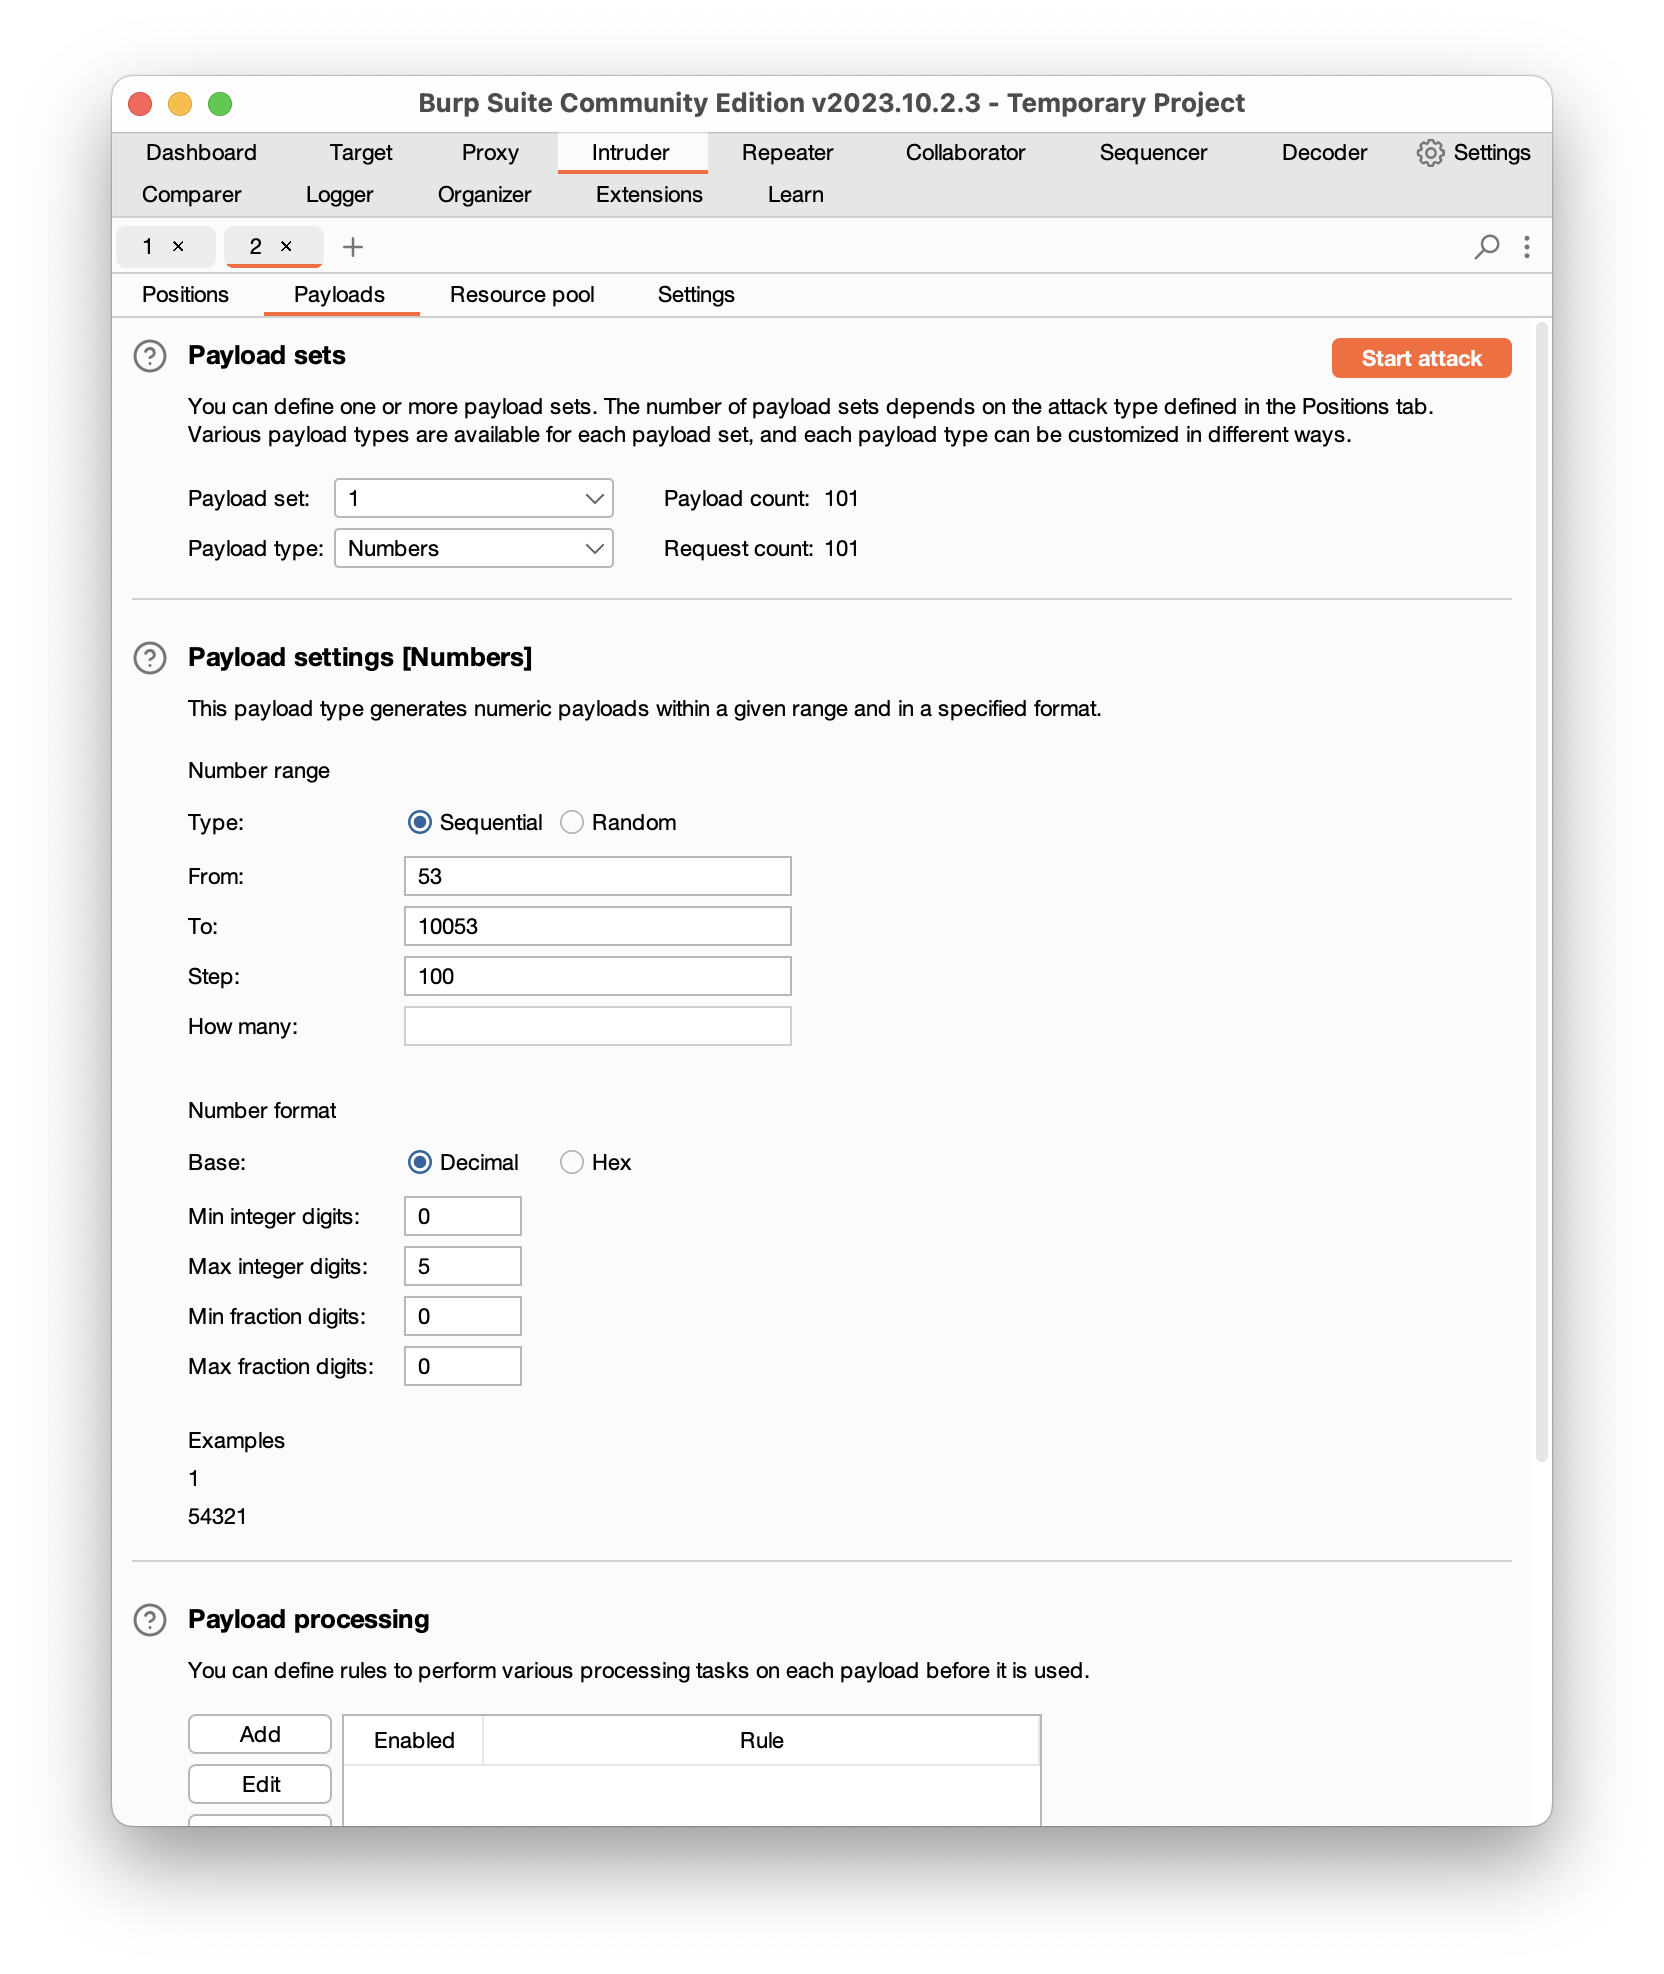
\includegraphics[width=14cm]{img/Web hacking/Beatles song catalogue/Skjermbilde 2023-10-26 kl. 13.06.47.png}
\end{center}

When the attack was done I searched through the results that had a length other than 232 or 233 since these were empty pages. I found the following page:

\begin{center}
    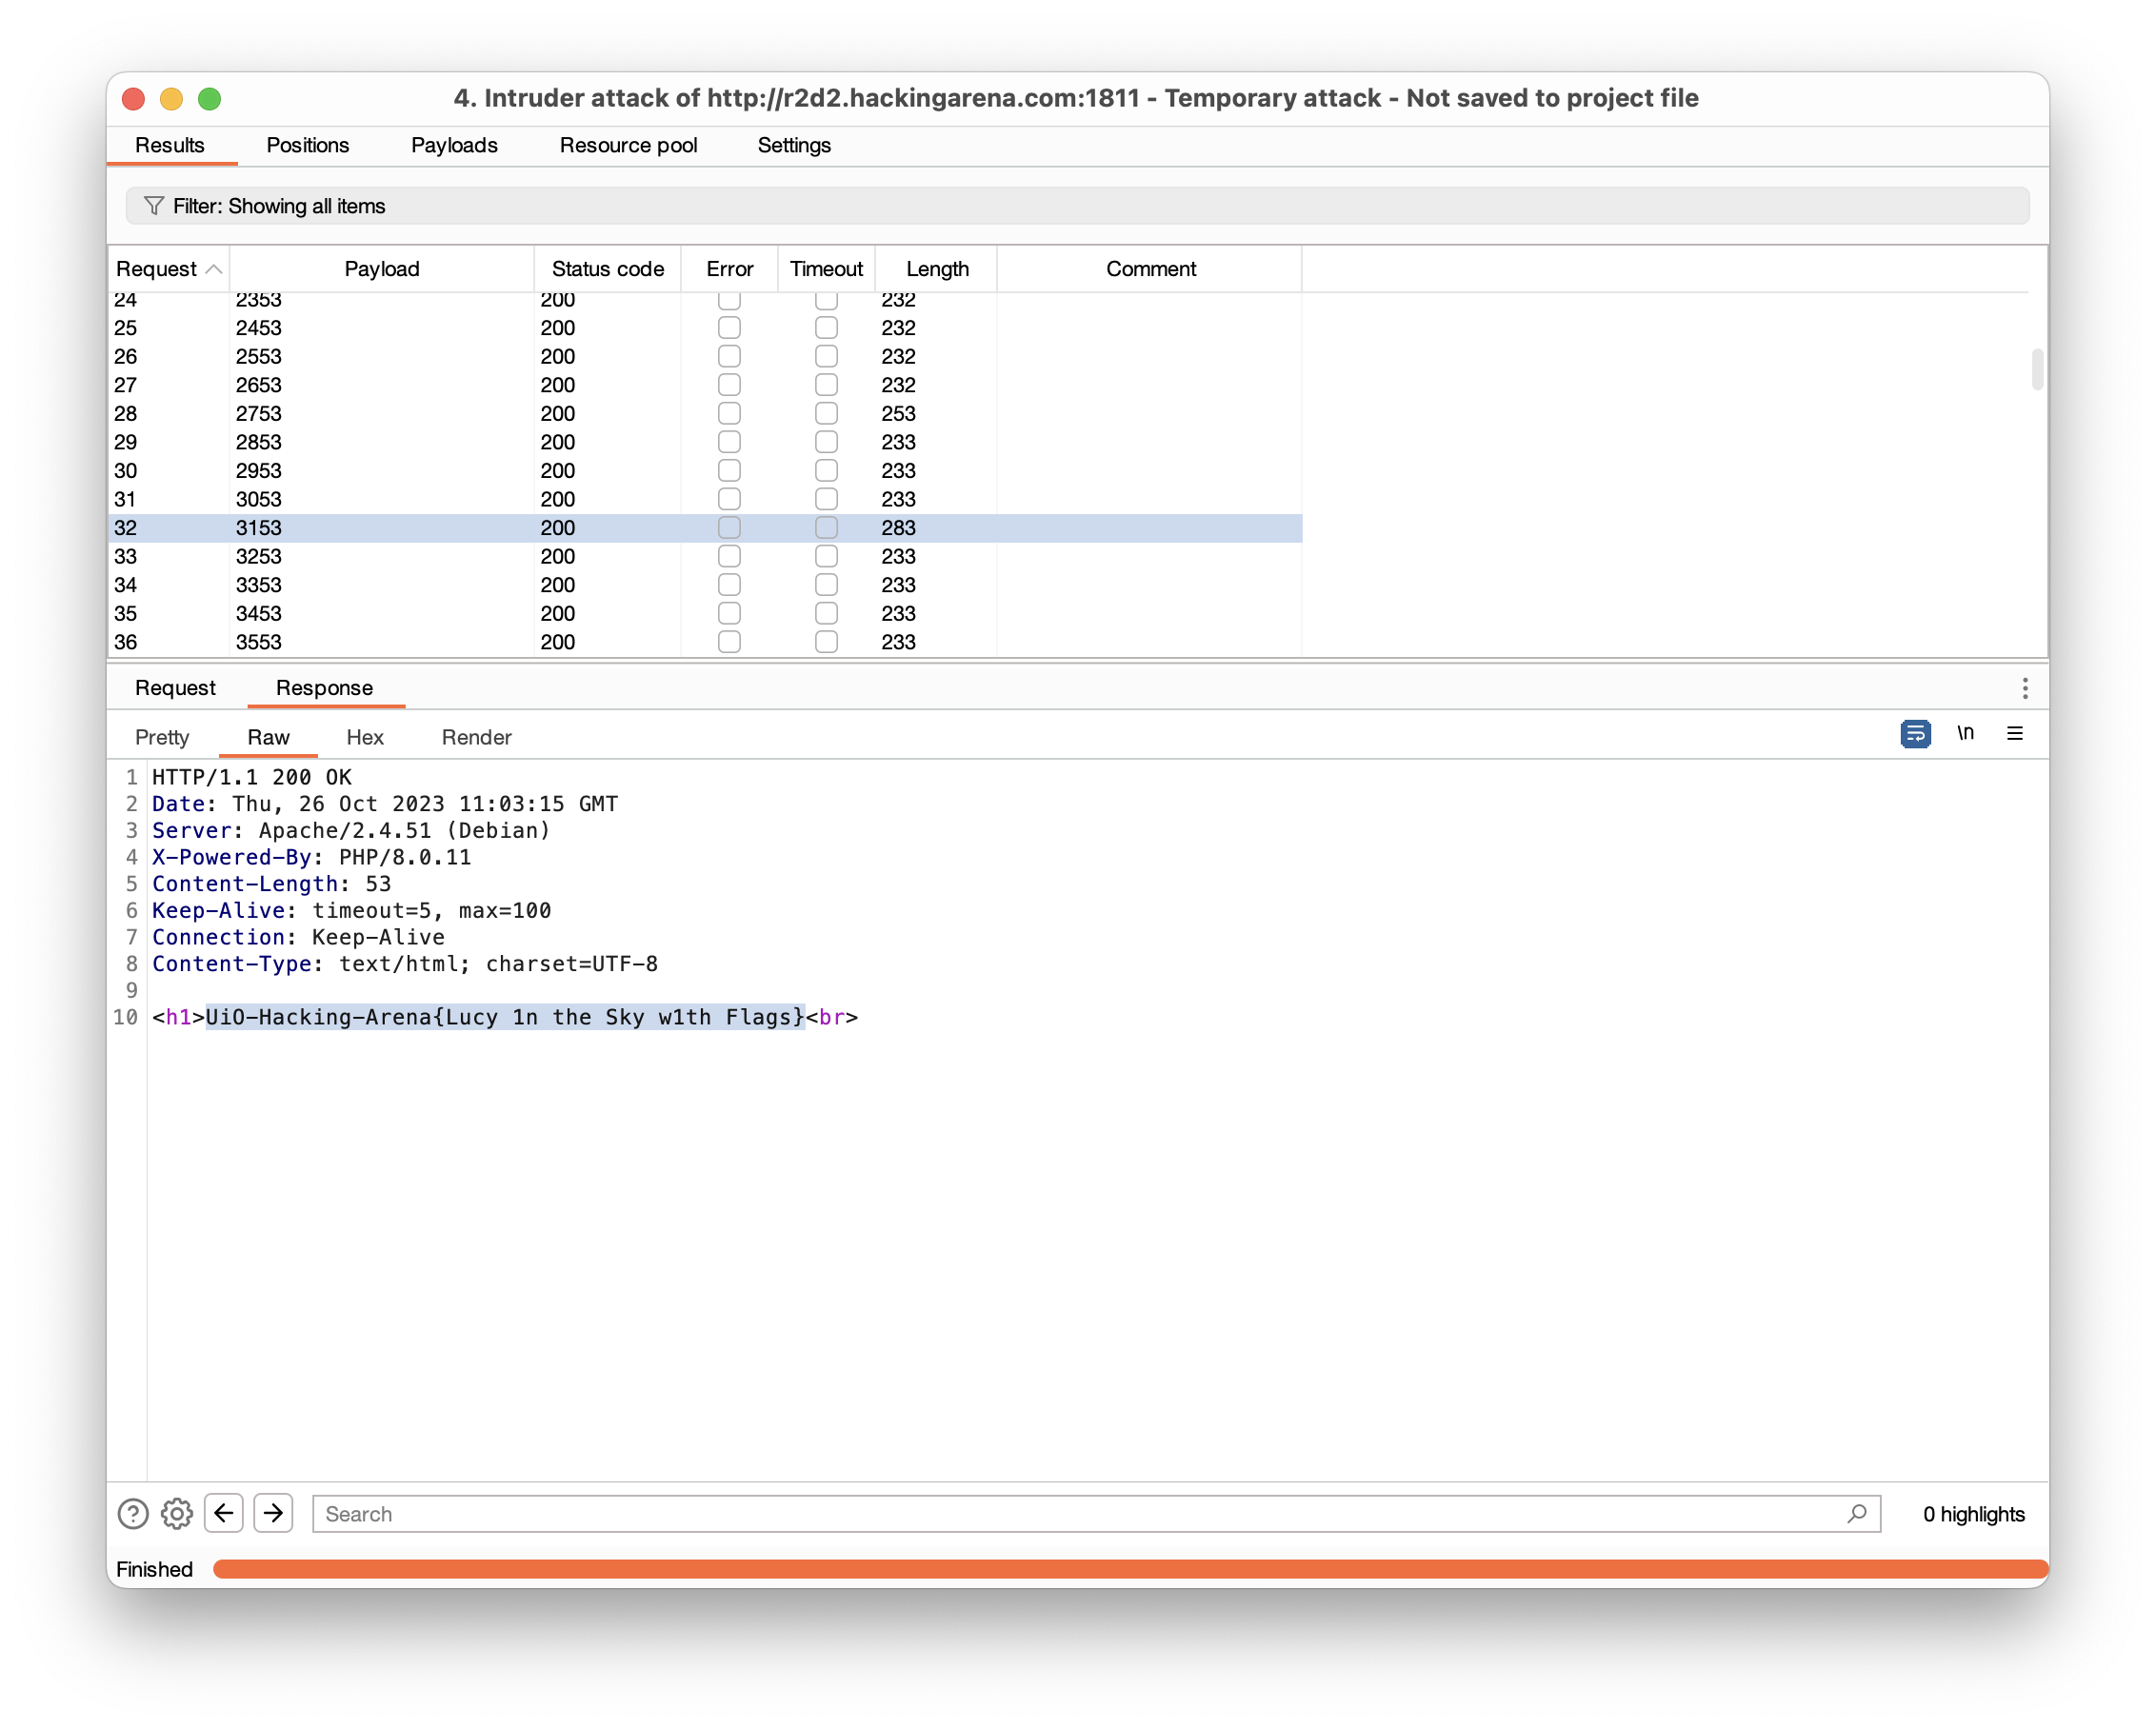
\includegraphics[width=15cm]{img/Web hacking/Beatles song catalogue/Skjermbilde 2023-10-26 kl. 13.06.58.png}
\end{center}

The flag is: \texttt{UiO-Hacking-Arena\string{Lucy 1n the Sky w1th Flags\string}}

\newpage
\subsection{Web 5 (60p)}
Can you find the flag here?
\url{http://padawan.hackingarena.com:820}

\textbf{Solution:}\\
The trick I found to solving this task was exceeding the character limit of the input field. When I did this I got the following error message:

\begin{center}
    
\includegraphics[width=12cm]{img/Web hacking/Web 5/Skjermbilde 2023-10-26 kl. 13.37.52.png}
\end{center}

Assuming the site was located at \texttt{/var/www/} I followed the path \texttt{partnerprocess/process.php}

\begin{center}
    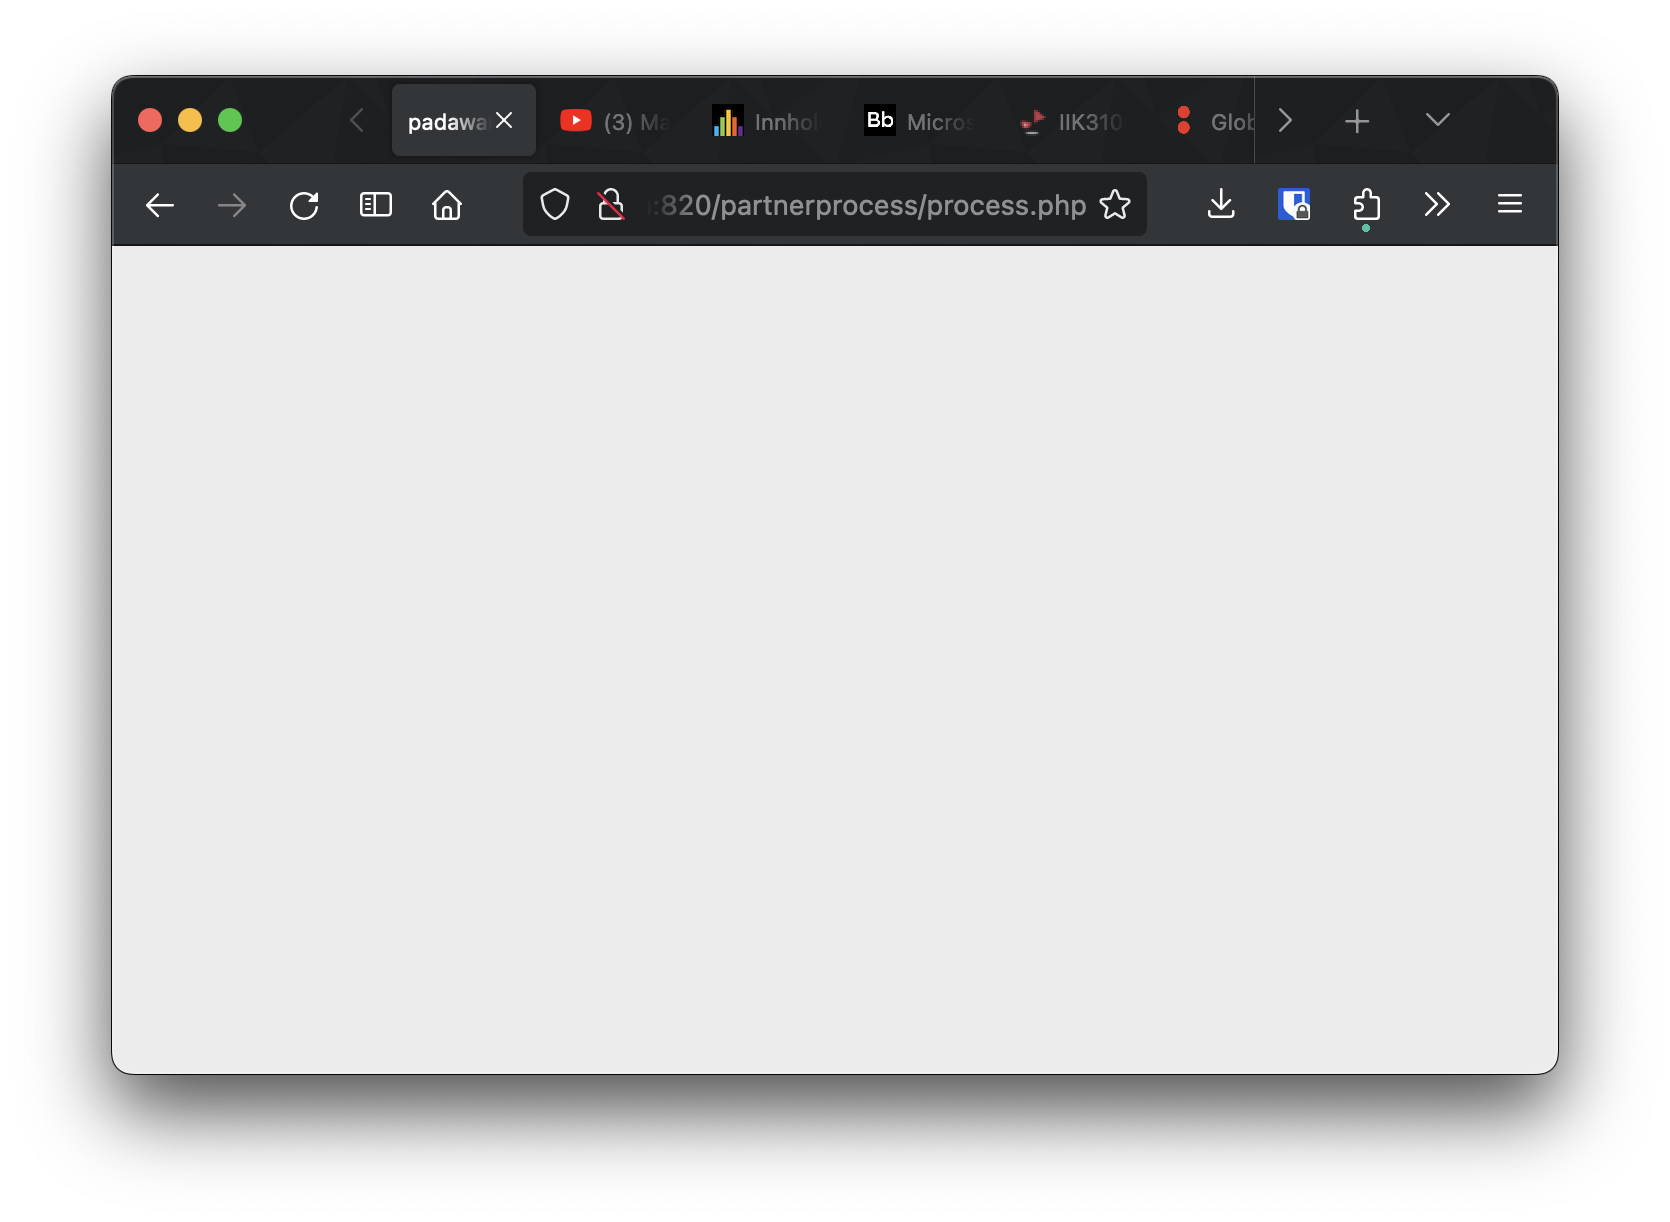
\includegraphics[width=12cm]{img/Web hacking/Web 5/Skjermbilde 2023-10-26 kl. 13.38.18.png}
\end{center}

After that I jumped to the parent directory \texttt{partnerprocess/} and found the flag in the \texttt{flag.txt} file.

\begin{center}
    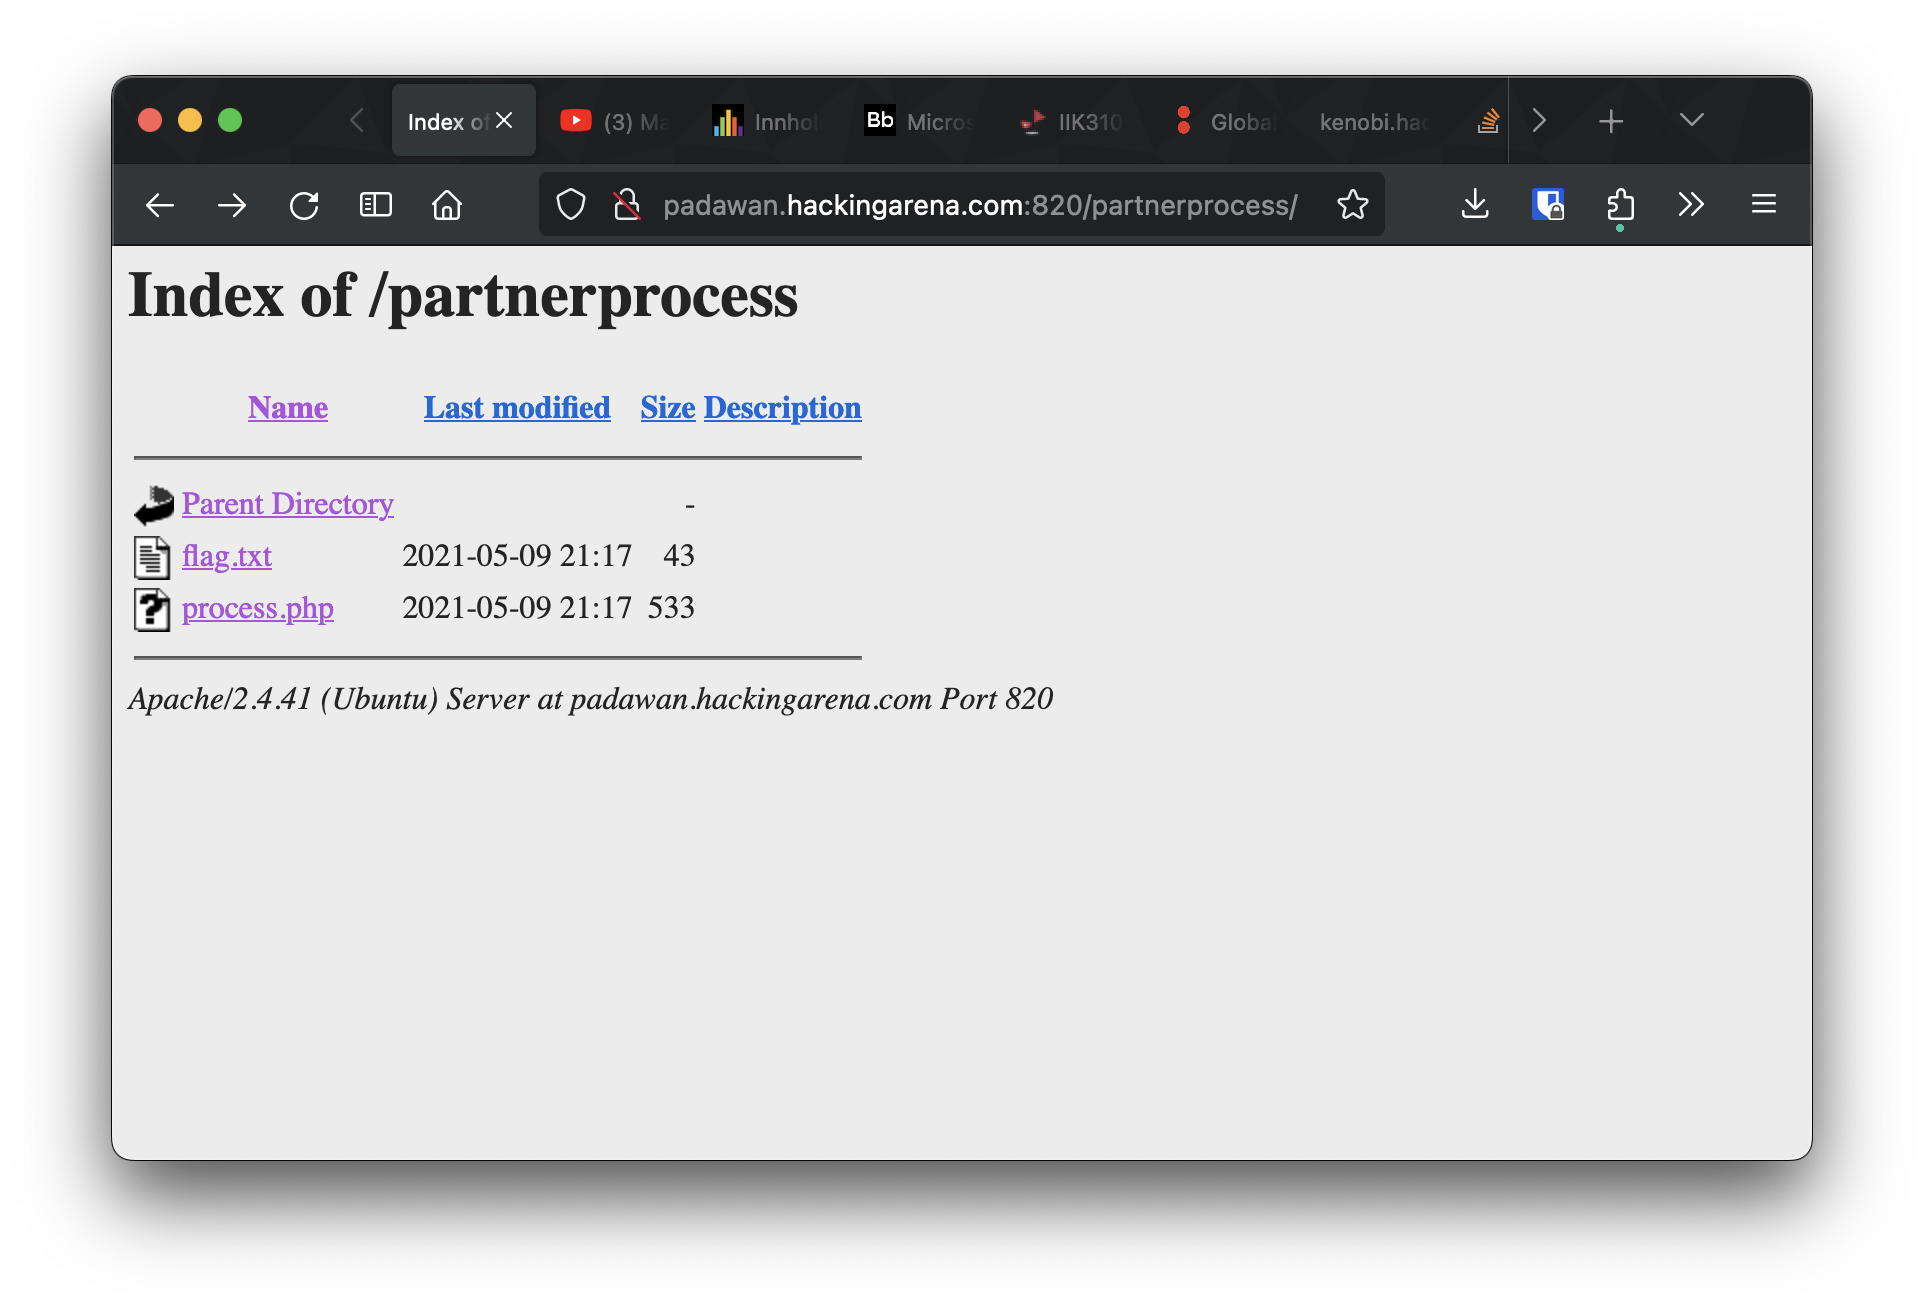
\includegraphics[width=12cm]{img/Web hacking/Web 5/Skjermbilde 2023-10-26 kl. 13.37.19.png}
\end{center}

Opening the file revealed the flag:

\begin{center}
    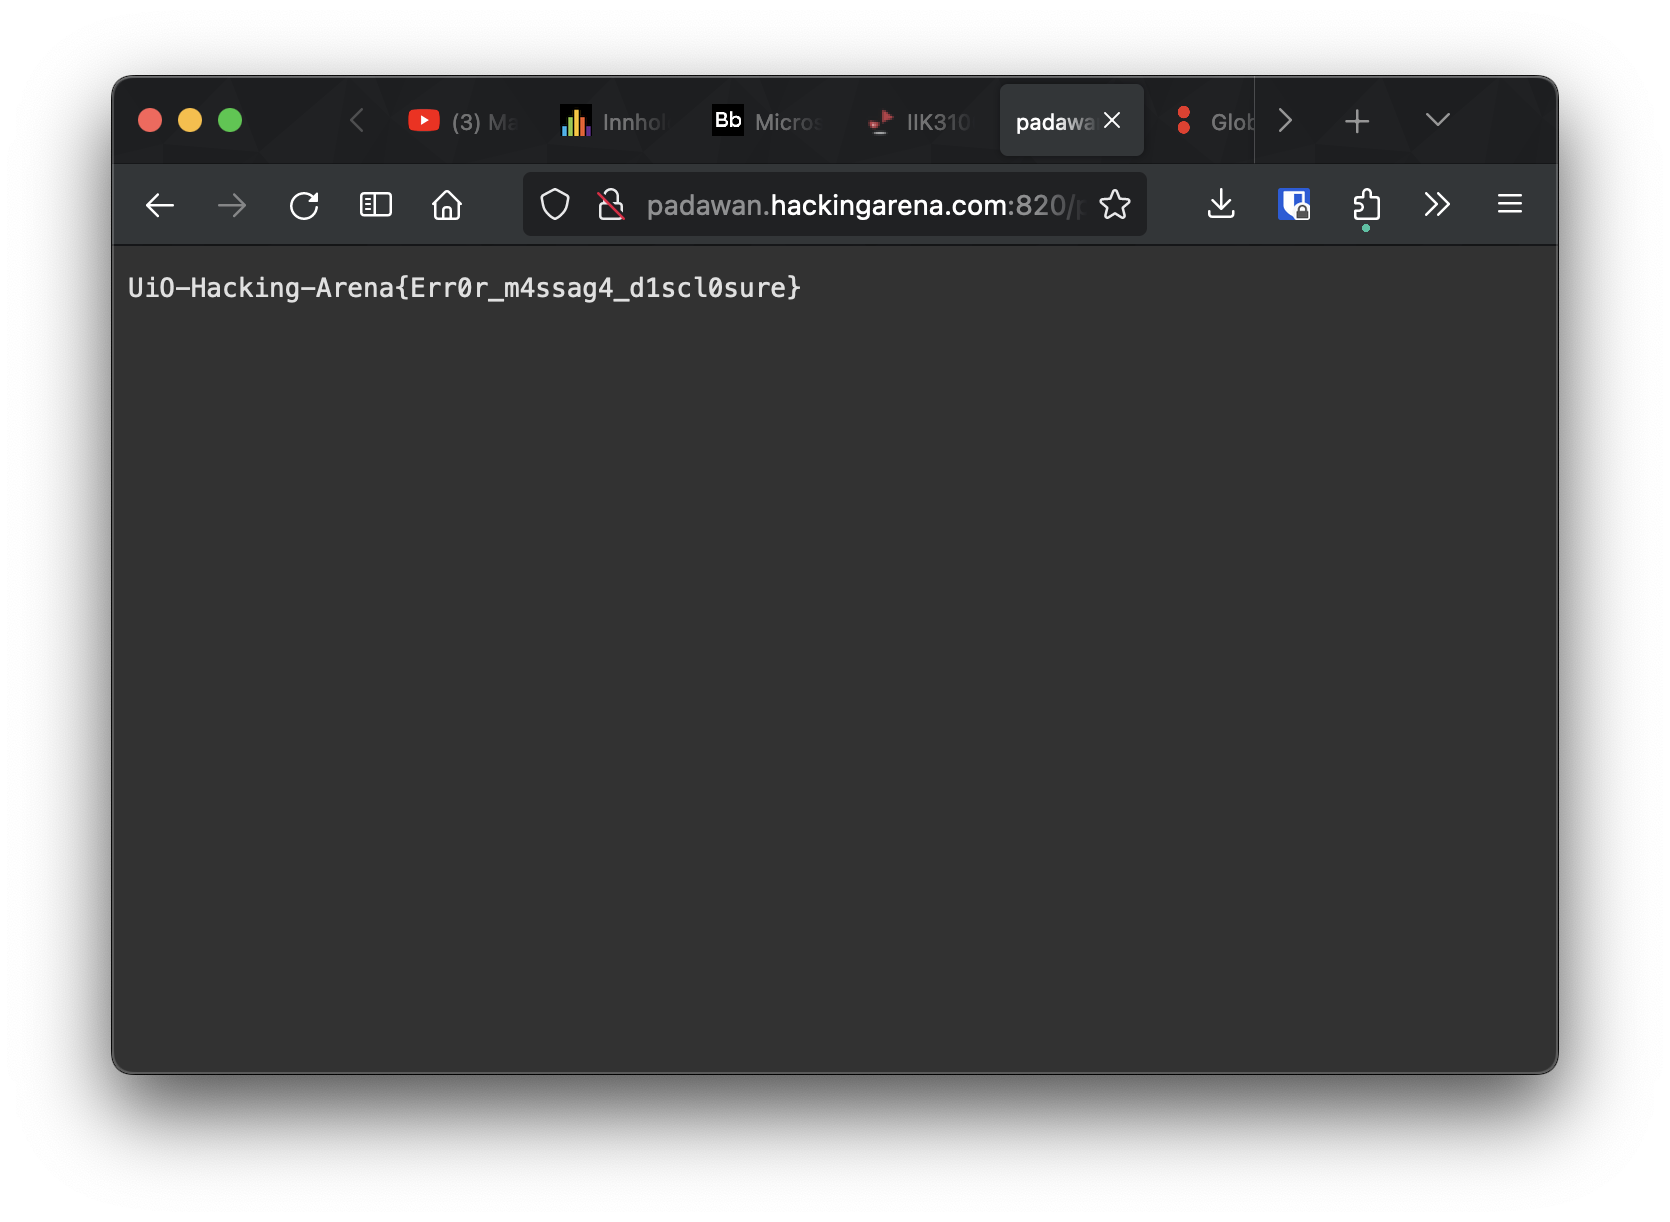
\includegraphics[width=12cm]{img/Web hacking/Web 5/Skjermbilde 2023-10-26 kl. 13.39.25.png}
\end{center}

The flag is: \texttt{UiO-Hacking-Arena\string{Err0r\_m4ssag4\_d1scl0sure\string}}

\newpage
\subsection{Redirect (60p)}
Can you redirect \texttt{kenobi.hackingarena.com:821} to \texttt{kenobi.hackingarena.com:822}?

\textbf{Solution:}\\
This task was all about cross site scripting. I first tried to inject a script into the input field, but this did not work. 
I then tried to log to the console with the injected script, but I realized some anti tampering mechanism was in place as I got a lot of \texttt{***ANTIHACKER***} in my log. 
I then had the idea of replacing the \texttt{window.location} with the new url.
This didn't work when injecting the script, so I tried again but this time in the console and it worked.

\begin{figure}[H]
    \centering
    \begin{minipage}{.5\textwidth}
        \hspace*{-1cm}
        \centerline{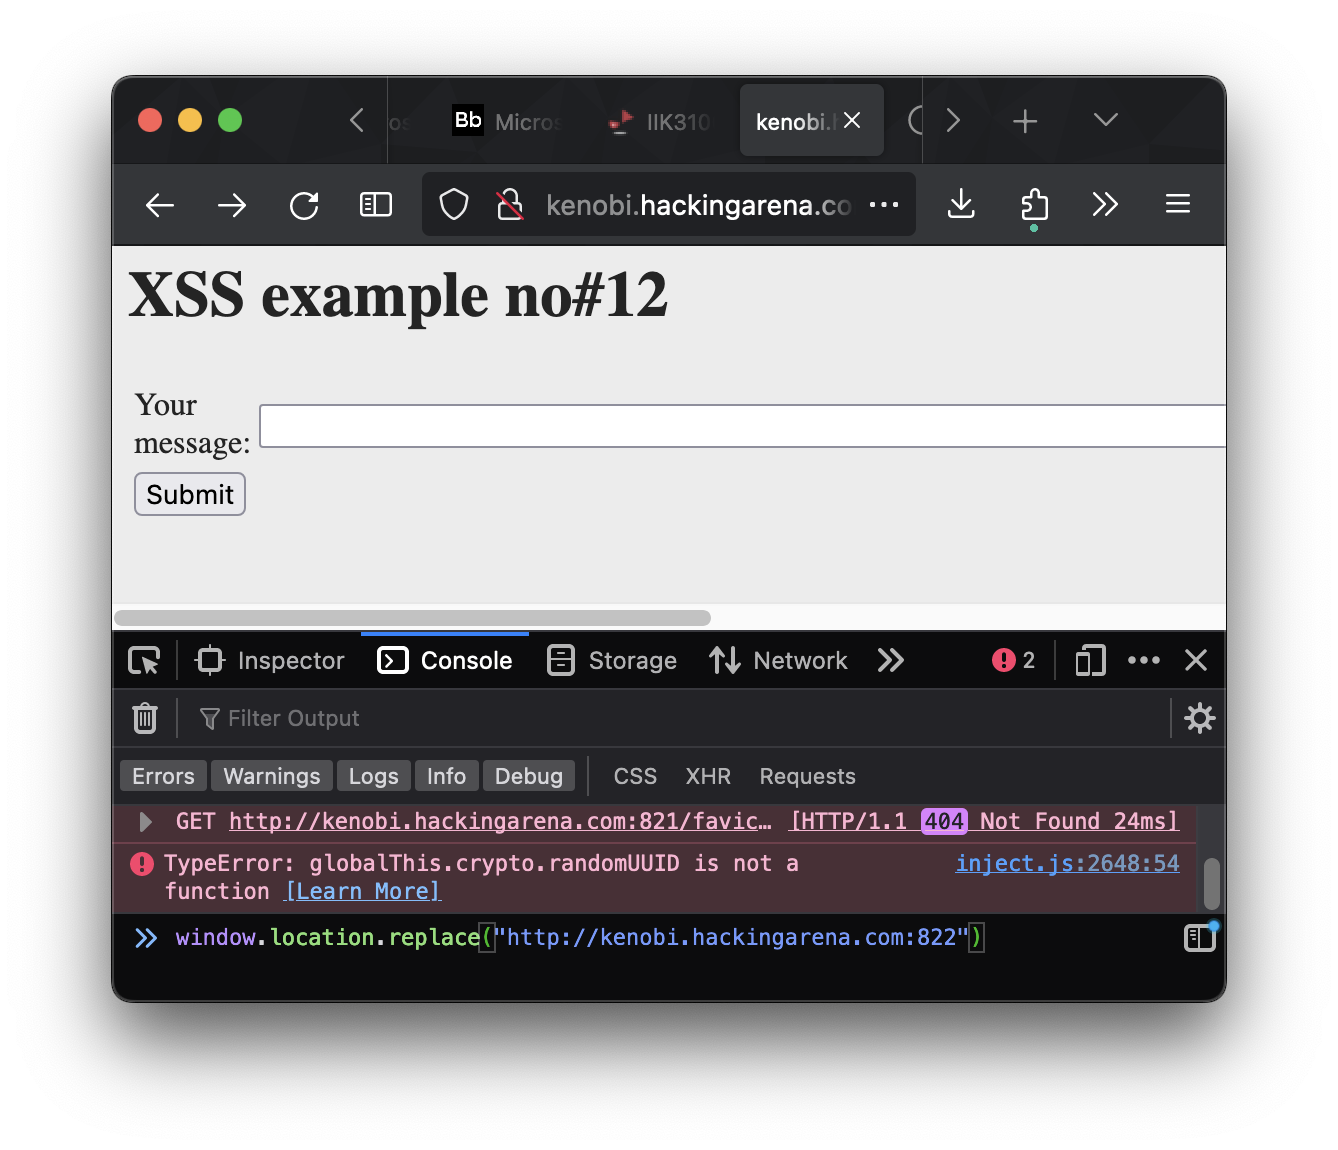
\includegraphics[width=1.4\textwidth]{img/Web hacking/Redirect/Skjermbilde 2023-10-26 kl. 15.29.27.png}}
        \vspace*{-.5cm}
        \captionof*{figure}{Before running the \\command in the console}
    \end{minipage}%
    \begin{minipage}{.5\textwidth}
        \hspace*{1cm}
        \centerline{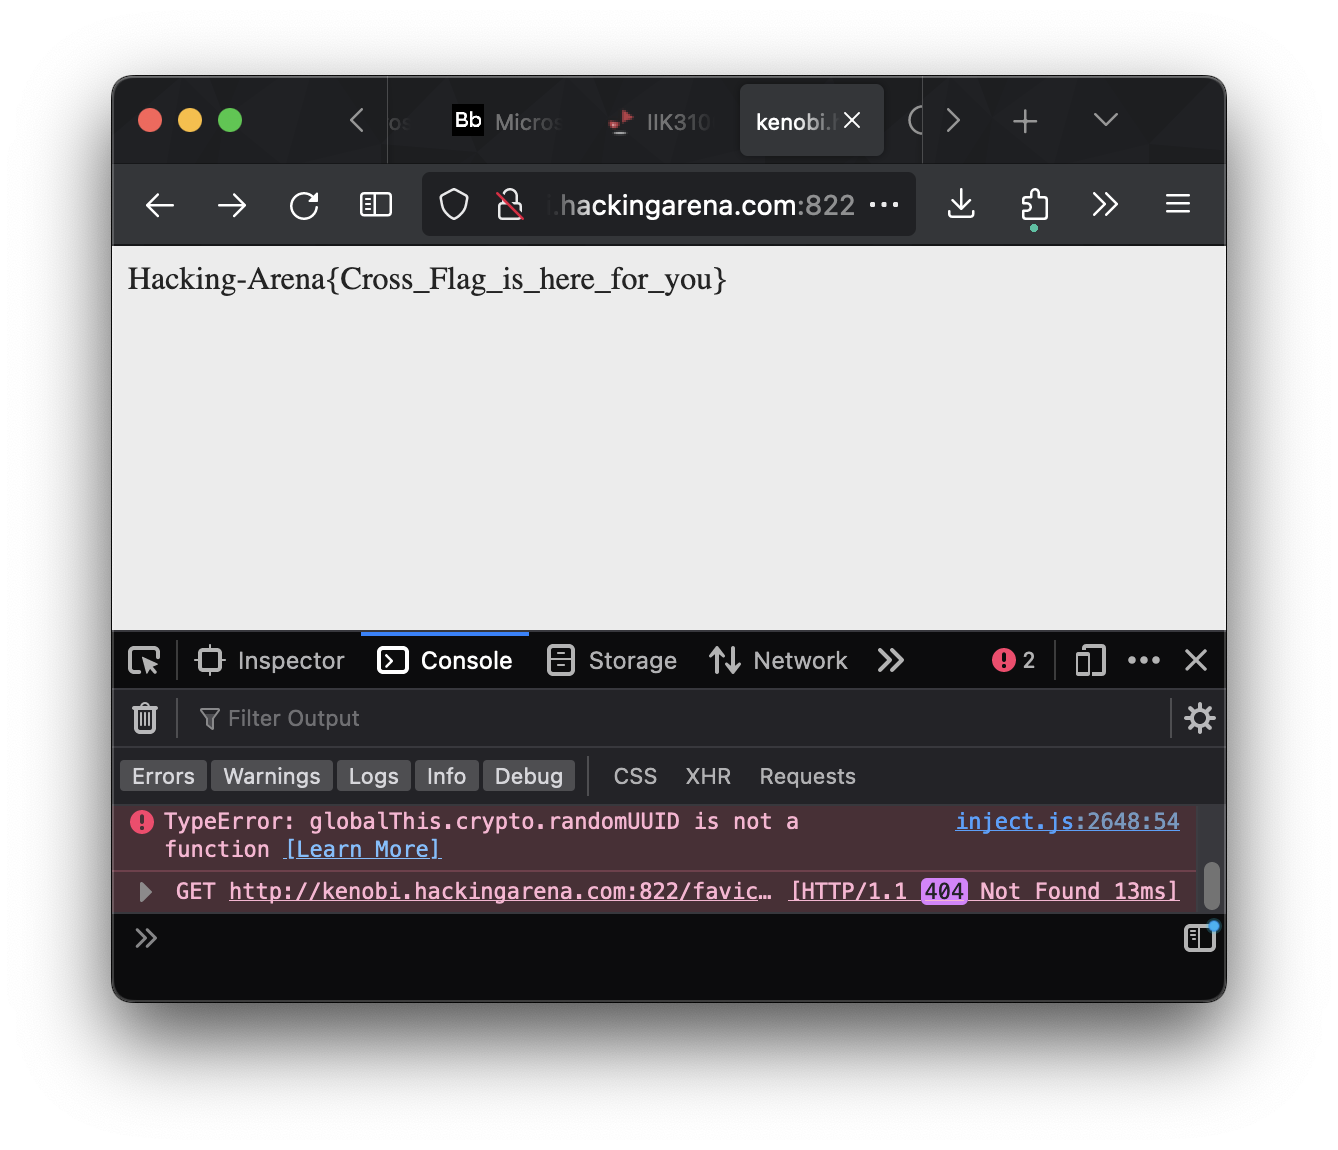
\includegraphics[width=1.4\textwidth]{img/Web hacking/Redirect/Skjermbilde 2023-10-26 kl. 15.29.41.png}}
        \vspace*{-1 cm}
        \captionof*{figure}{After running the \\command in the console}
    \end{minipage}
\end{figure}

\newpage
\subsection{Arenabook (80p)}
Hi, Check out the latest social media platform:
\url{http://sidious.hackingarena.com:803}
Sandra already tried it. :)

\textbf{Solution:}\\
The first step was to look for Sandra.

\begin{center}
    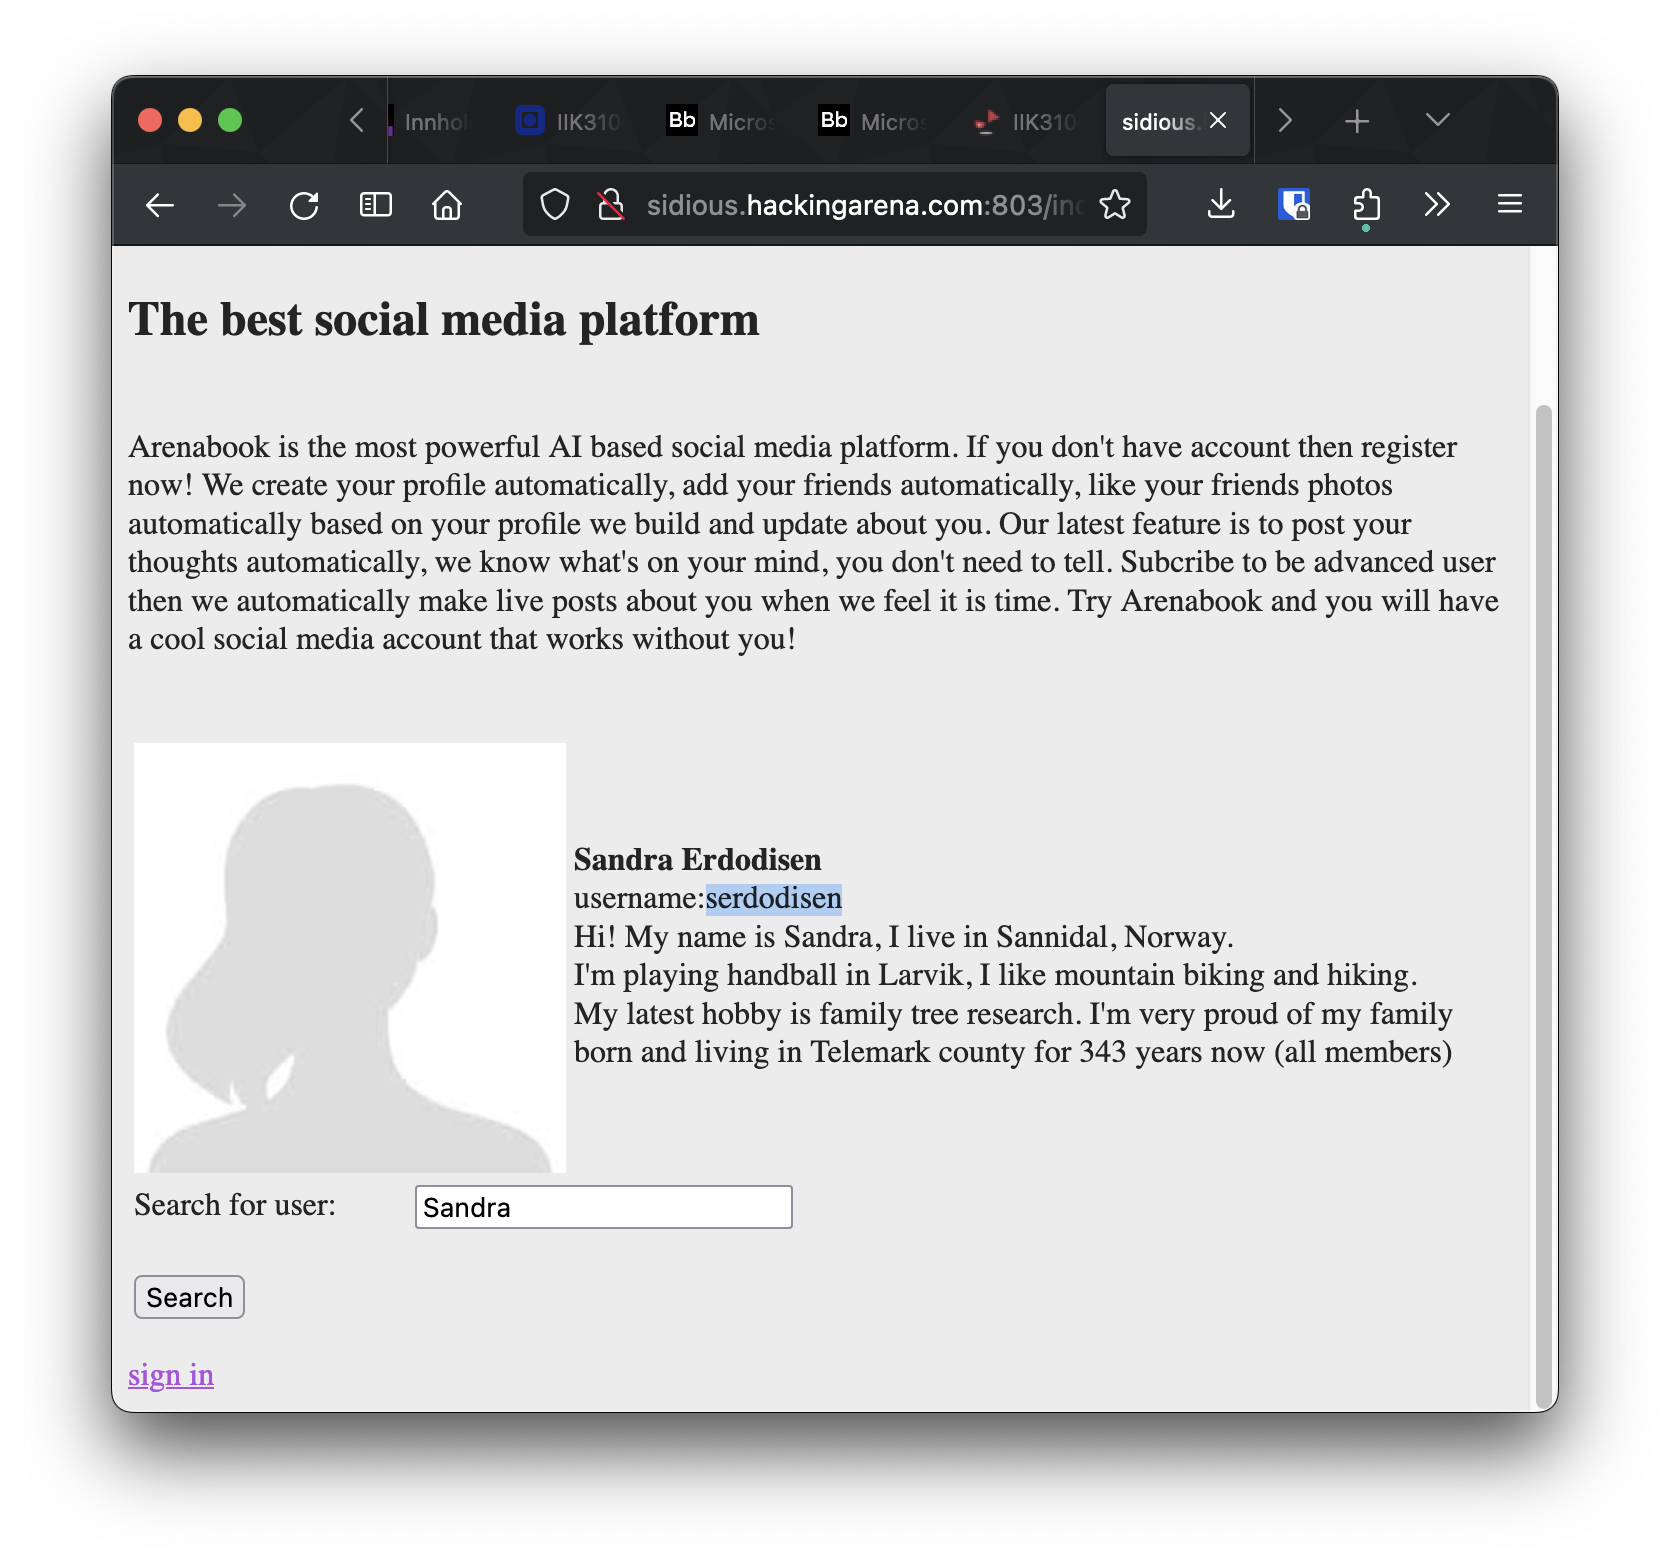
\includegraphics[width=15cm]{img/Web hacking/Arenabook/Skjermbilde 2023-10-26 kl. 14.49.43.png}
\end{center}

After getting her username I could use the forgot password function to get her password. I ended up at a page asking for the birthplace of her grandmother.

\begin{center}
    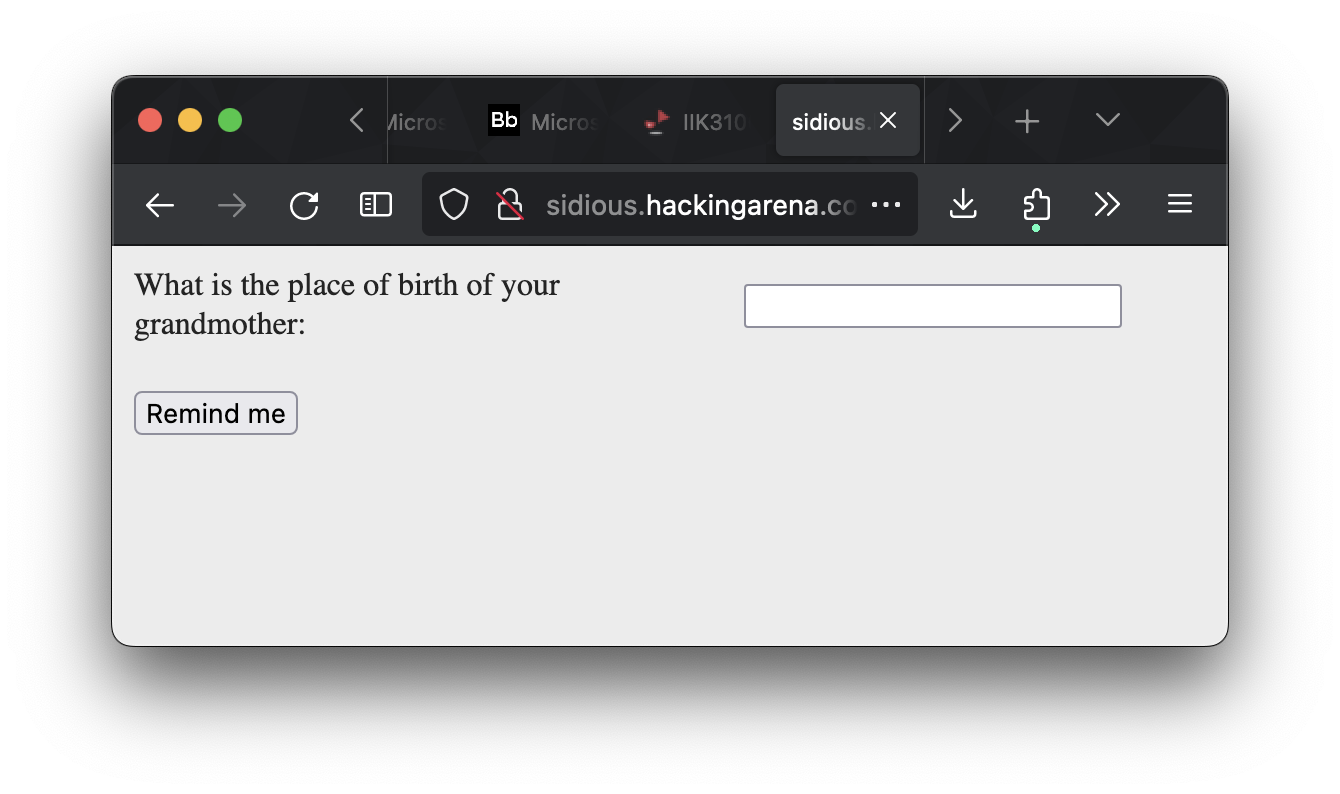
\includegraphics[width=14cm]{img/Web hacking/Arenabook/Skjermbilde 2023-10-26 kl. 14.50.02.png}
\end{center}

After putting the page into Burp Suite I found a field where different place names could be tried.
I then visited the Wikipedia page <<\href{https://en.wikipedia.org/wiki/List_of_villages_in_Telemark}{List of villages in Telemark}>> and downloaded the list of villages to a text file.
Then in Burp Suite I set up an intruder attack with the list of villages as the payload.

\begin{center}
    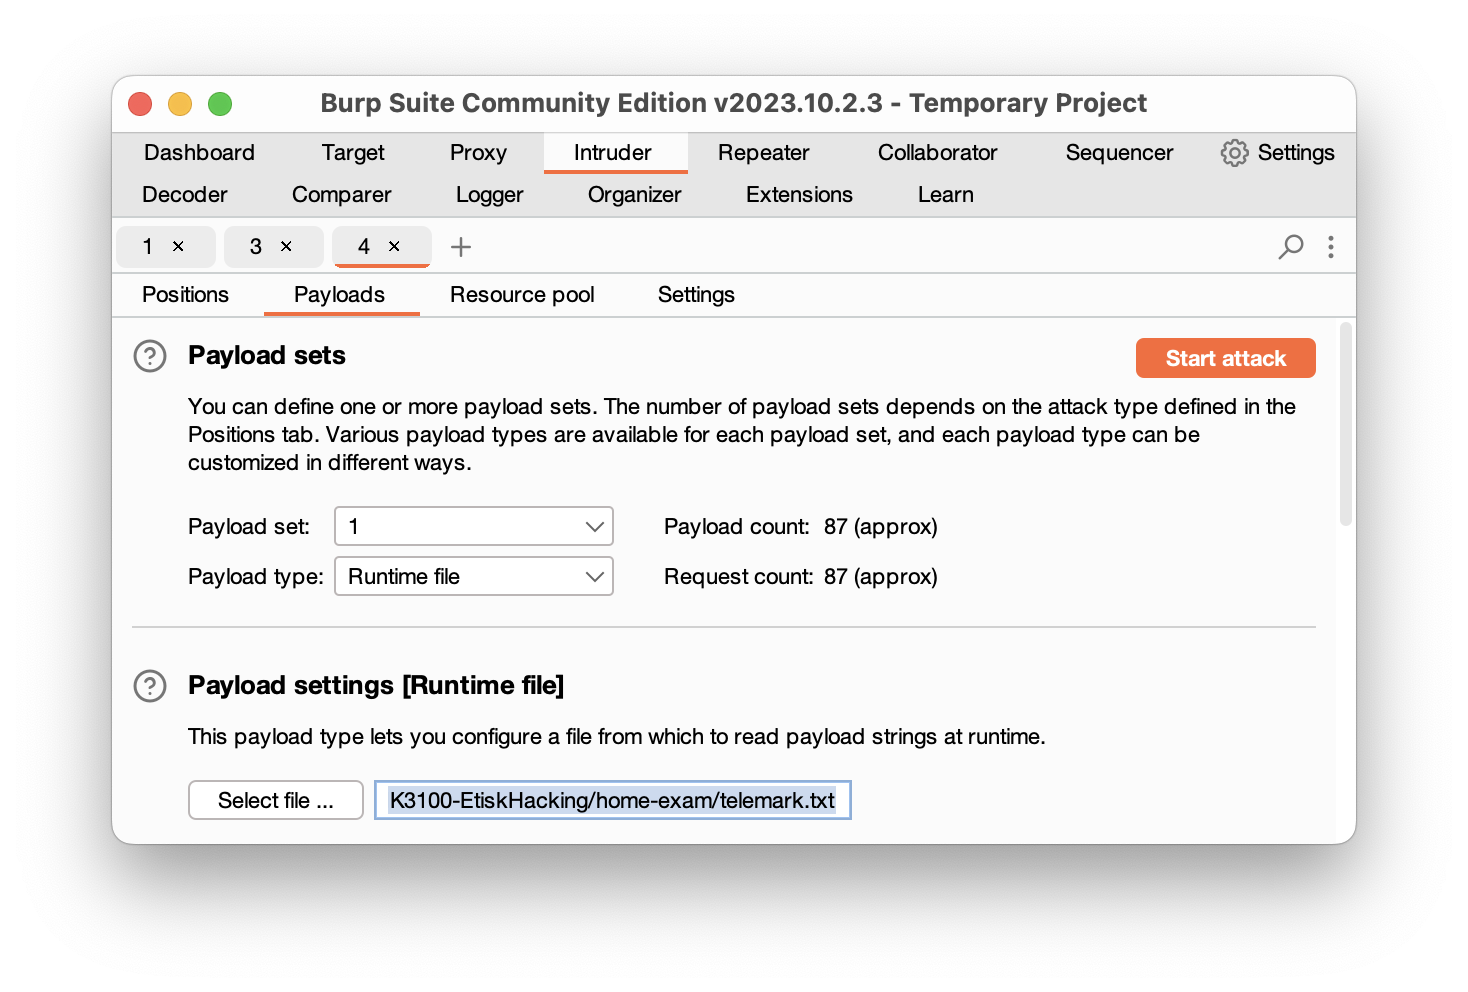
\includegraphics[width=15cm]{img/Web hacking/Arenabook/Skjermbilde 2023-10-26 kl. 14.54.29.png}
\end{center}

After the attack was done I searched through the results and found the following page:

\begin{center}
    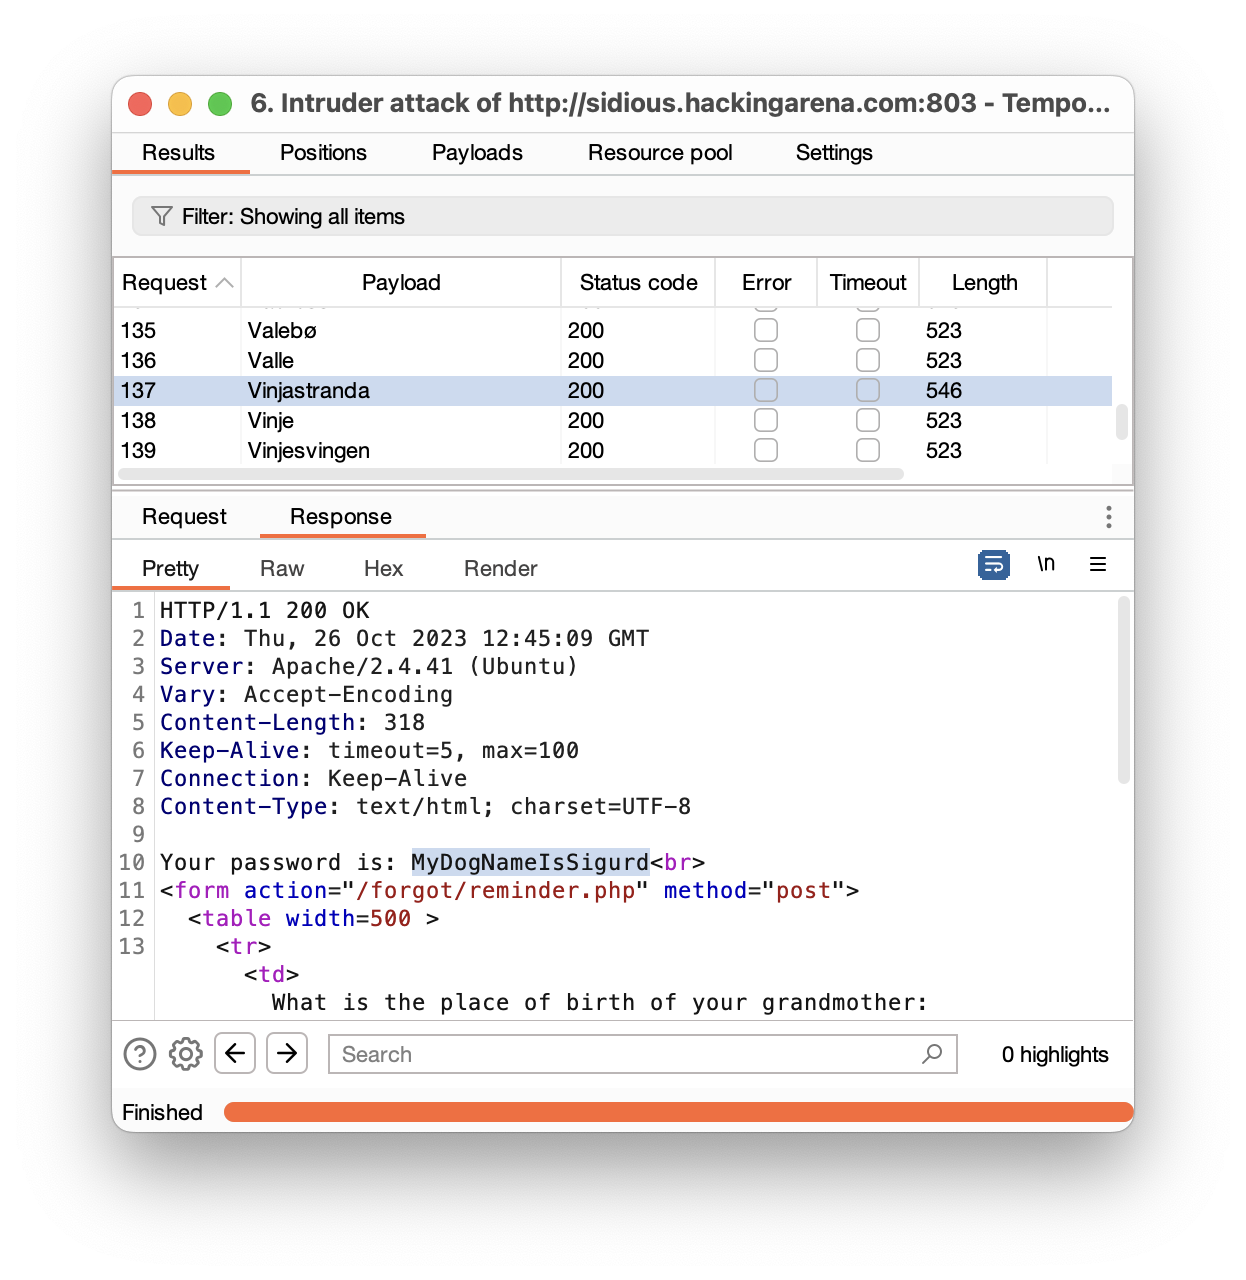
\includegraphics[width=13cm]{img/Web hacking/Arenabook/Skjermbilde 2023-10-26 kl. 14.55.08.png}
\end{center}

Sandras grandmother was born in \texttt{Vinjastranda}, and her password was \texttt{MyDogNameIsSigurd}. Using the password I could log in to Sandras account and get the flag.

\begin{center}
    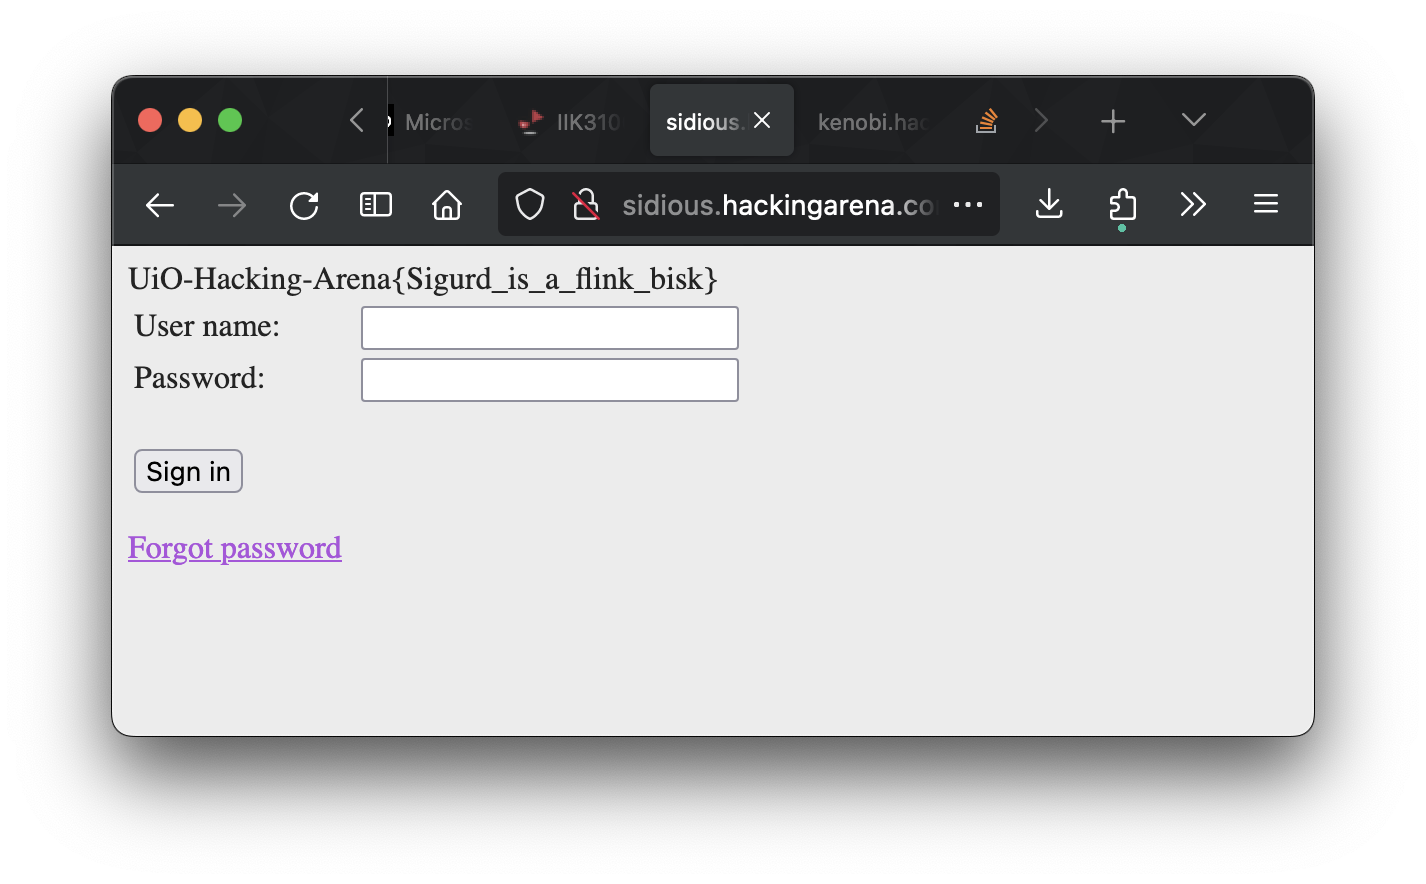
\includegraphics[width=12cm]{img/Web hacking/Arenabook/Skjermbilde 2023-10-26 kl. 14.55.36.png}
\end{center}

\subsection{Cybersmart (80p)}
Find the flag here: \url{http://padawan.hackingarena.com:804}

\textbf{Solution:}\\

When first entering the site I clicked on the \texttt{CyberSmart} link and noticed that the url had changed and that i got some text output on the page.
After some trial and error I figured that the url parameter \texttt{program} executed a program from a directory. So I then naively tried to execute the \texttt{ls} command from the \texttt{/bin} directory.

\begin{center}
    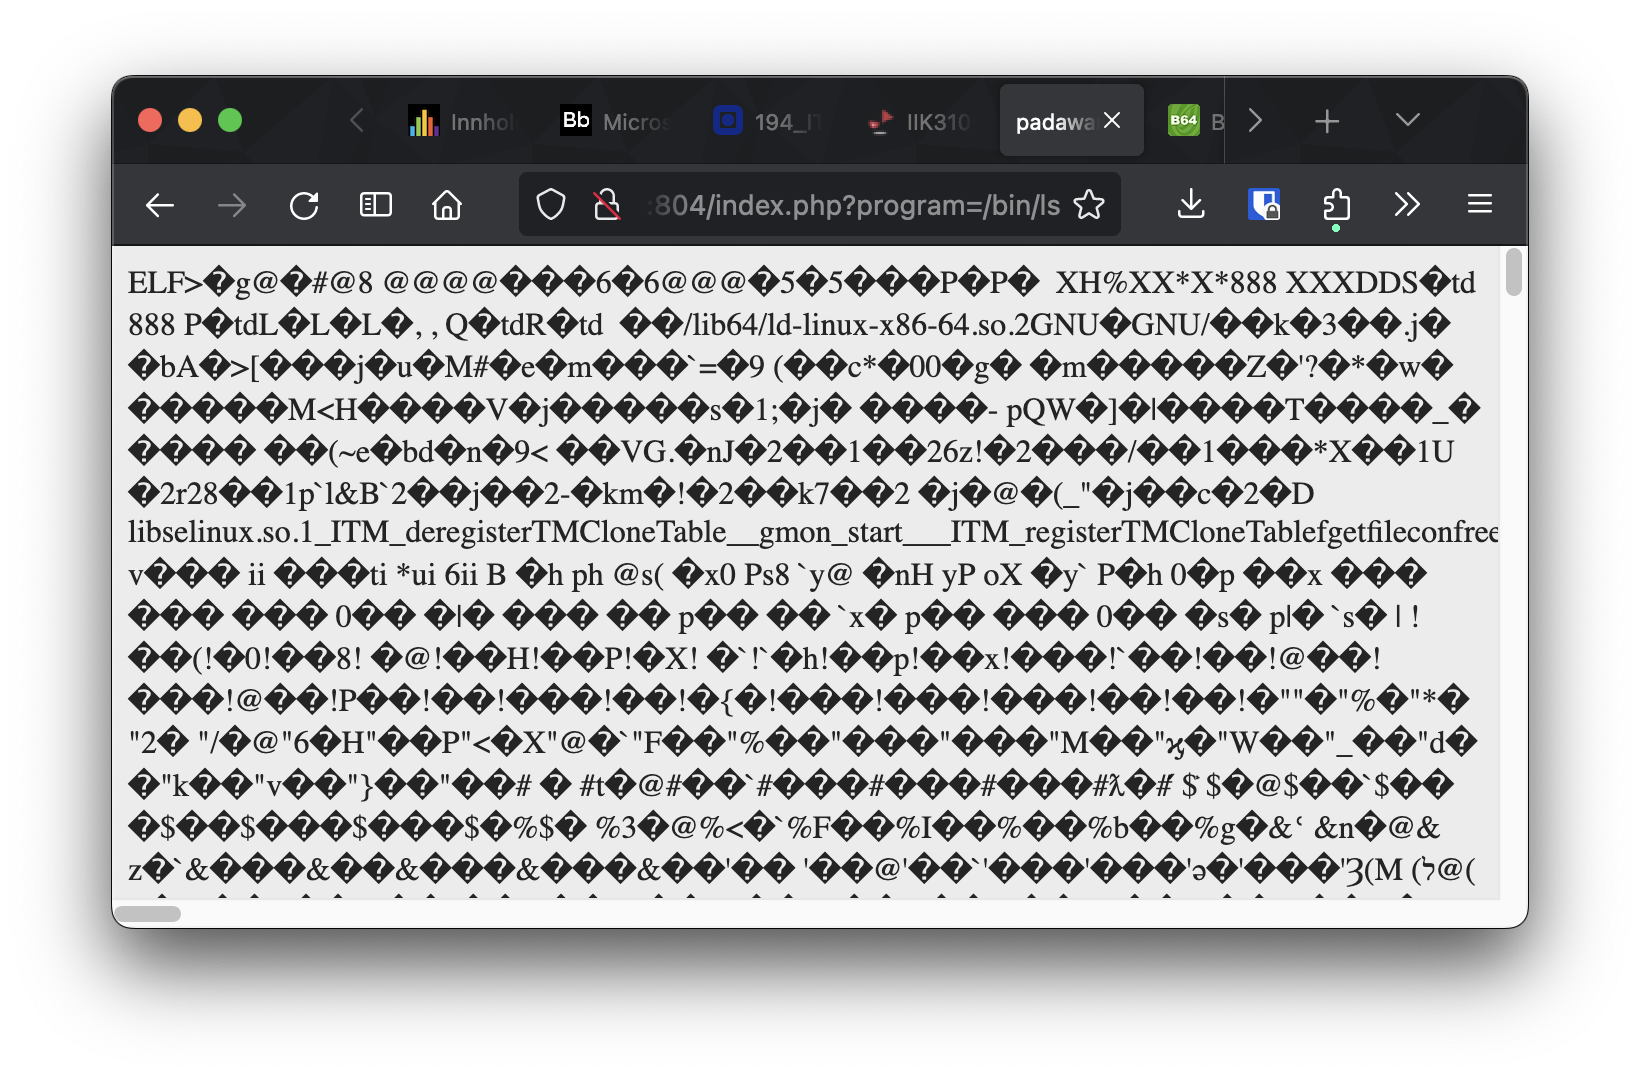
\includegraphics[width=12cm]{img/Web hacking/Cybersmart/Screenshot 2023-11-09 at 14.03.33.png}
\end{center}

Since that clearly didn't work I looked more into what to do and found that I could get the source code from the php script encoded in base64 by adding\\ \texttt{php://filter/convert.base64-encode/resource=index.php} to the program parameter.

\begin{center}
    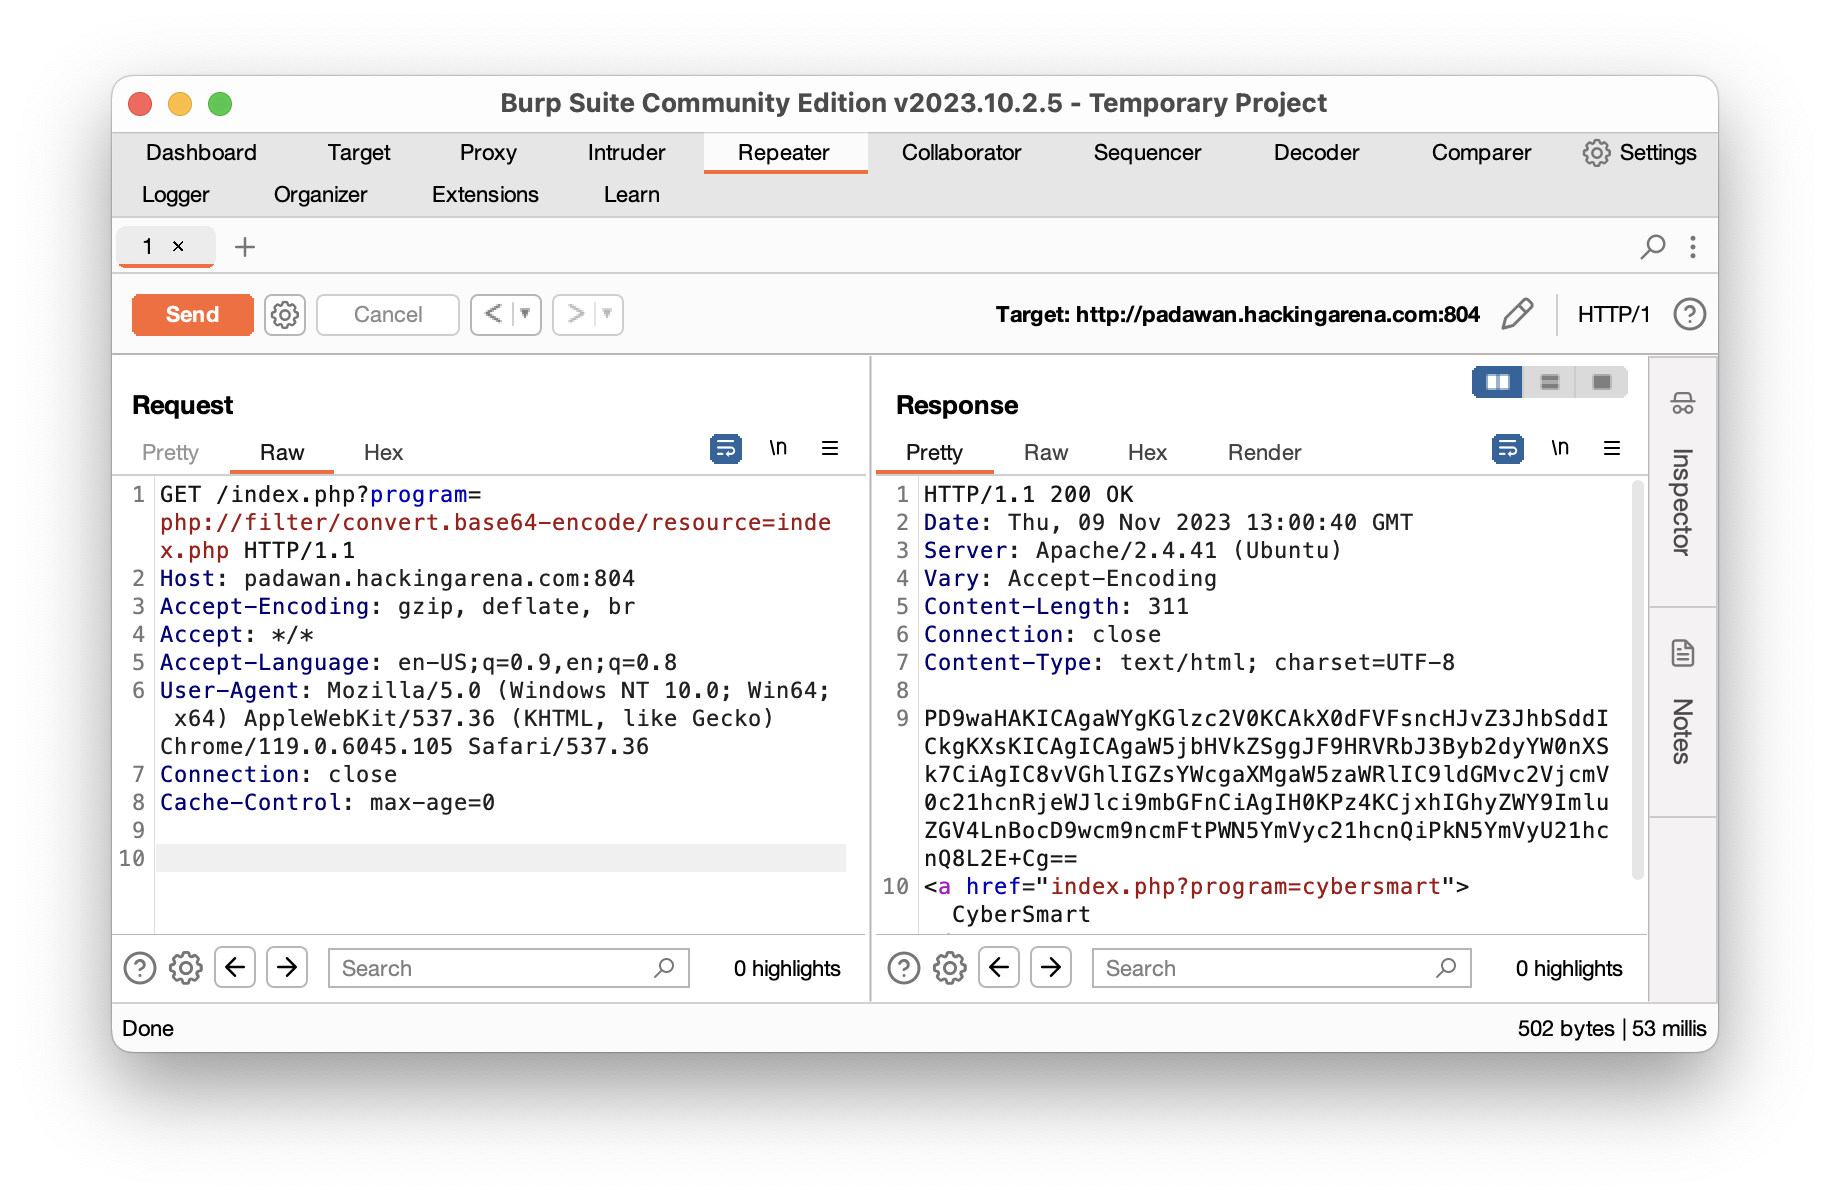
\includegraphics[width=12cm]{img/Web hacking/Cybersmart/Screenshot 2023-11-09 at 14.04.28.png}
\end{center}

I then decoded the base64 string and got the following code:

\begin{center}
    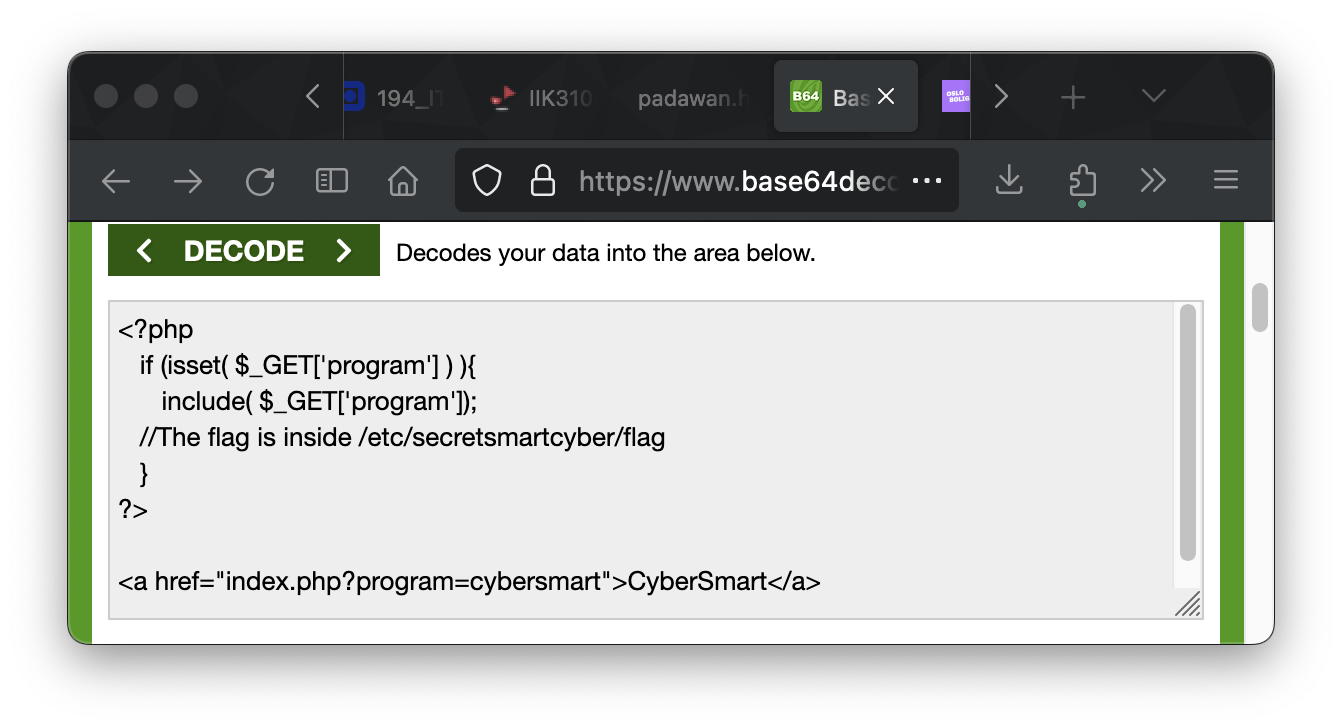
\includegraphics[width=15cm]{img/Web hacking/Cybersmart/Screenshot 2023-11-09 at 14.05.04.png}
\end{center}

In the code it told where the flag was located, so I located the file and got the following output:

\begin{center}
    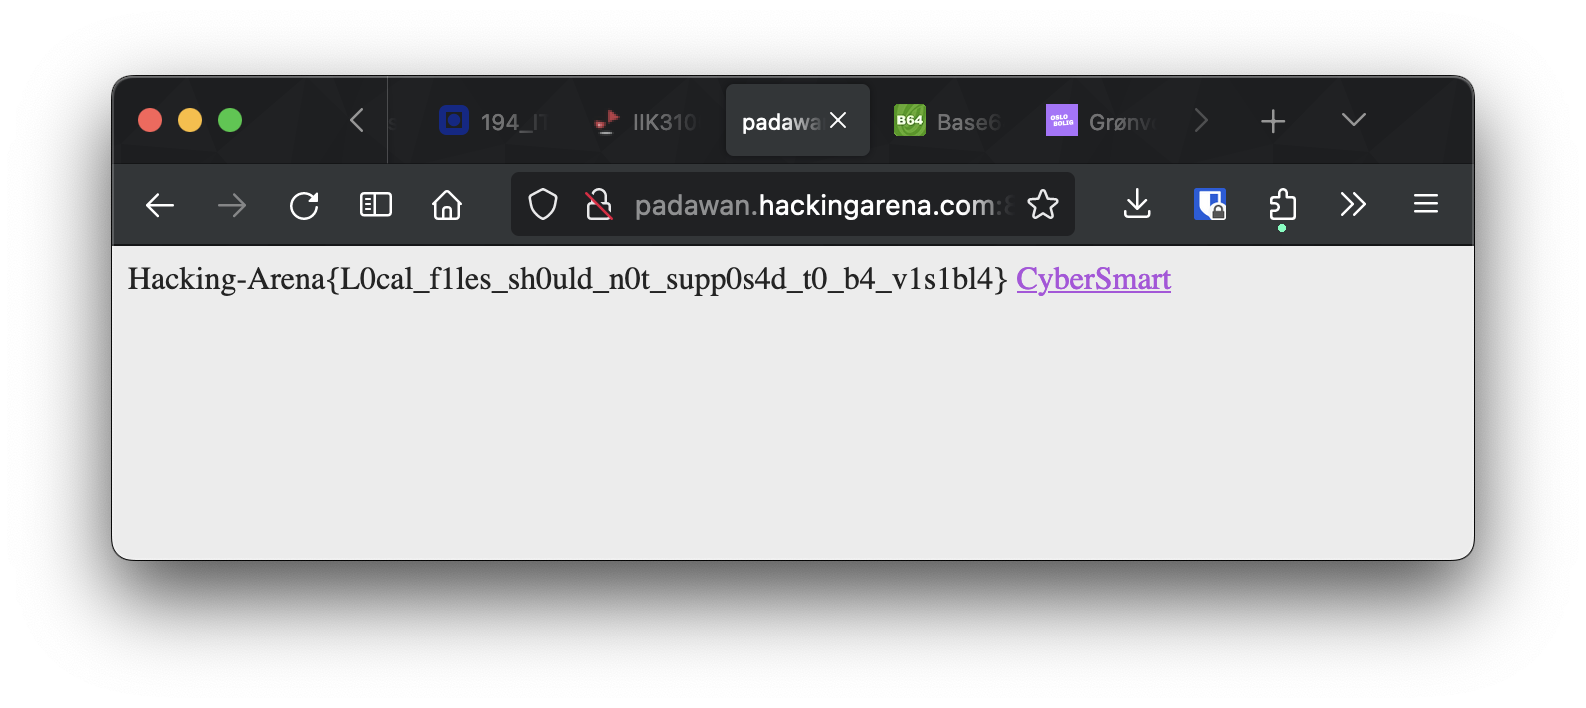
\includegraphics[width=15cm]{img/Web hacking/Cybersmart/Screenshot 2023-11-09 at 14.02.40.png}
\end{center}

The flag is: \texttt{Hacking-Arena\string{L0cal\_f1les\_sh0uld\_n0t\_supp0s4d\_t0\_b4\_v1s1bl4\string}}

\newpage
\subsection{Beatles song catalogue 2 (100p)}
Find the flag here: \url{http://r2d2.hackingarena.com:1819}

\textbf{Solution:}\\
The challenge in this task for me was to figure out what parameters to use and how to use them with sqlmap.
I started by using Burp Suite to find the parameters and cookies used by the site.
I first searched with the \texttt{song}, \texttt{user} and \texttt{pass} parameters, but I didn't get any results.
Then after realizing the select boxes also provided parameters I tried with the \texttt{year}, \texttt{vocal} and \texttt{album} parameters as well as the \texttt{city} parameter from the form that appeared after loggin in.
With that I used the following command to find the databases and tables:

\texttt{sqlmap -u "http://r2d2.hackingarena.com:1819/index.php?year=1964\&vocal=2\&album=3" --current-db --cookie="PHPSESSID=sb35apjt8vor4ud1c236sfus6i" --data="city=London\&year=1962\&song=Let" --tables}

That resulted in finding the database \texttt{BeatlesData} and the table \texttt{Flag}. 

\begin{center}
    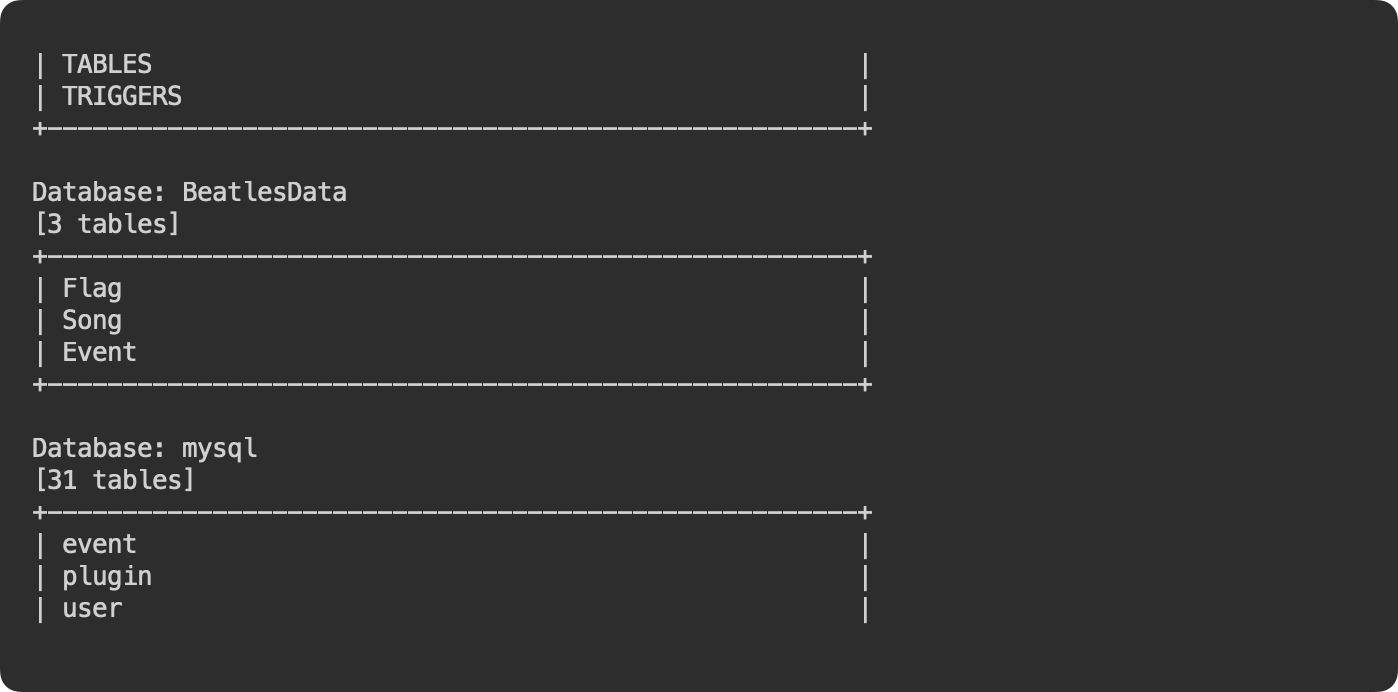
\includegraphics[width=15cm]{img/Web hacking/Beatles song catalogue 2/Screenshot 2023-11-10 at 14.10.27.png}
\end{center}

I then dumped the table with the following command:

\texttt{sqlmap -u "http://r2d2.hackingarena.com:1819/index.php?year=1964" --current-db --cookie="PHPSESSID=sb35apjt8vor4ud1c236sfus6i"  --tables -D BeatlesData -T Flag --dump}

That gave me the following output:

\begin{center}
    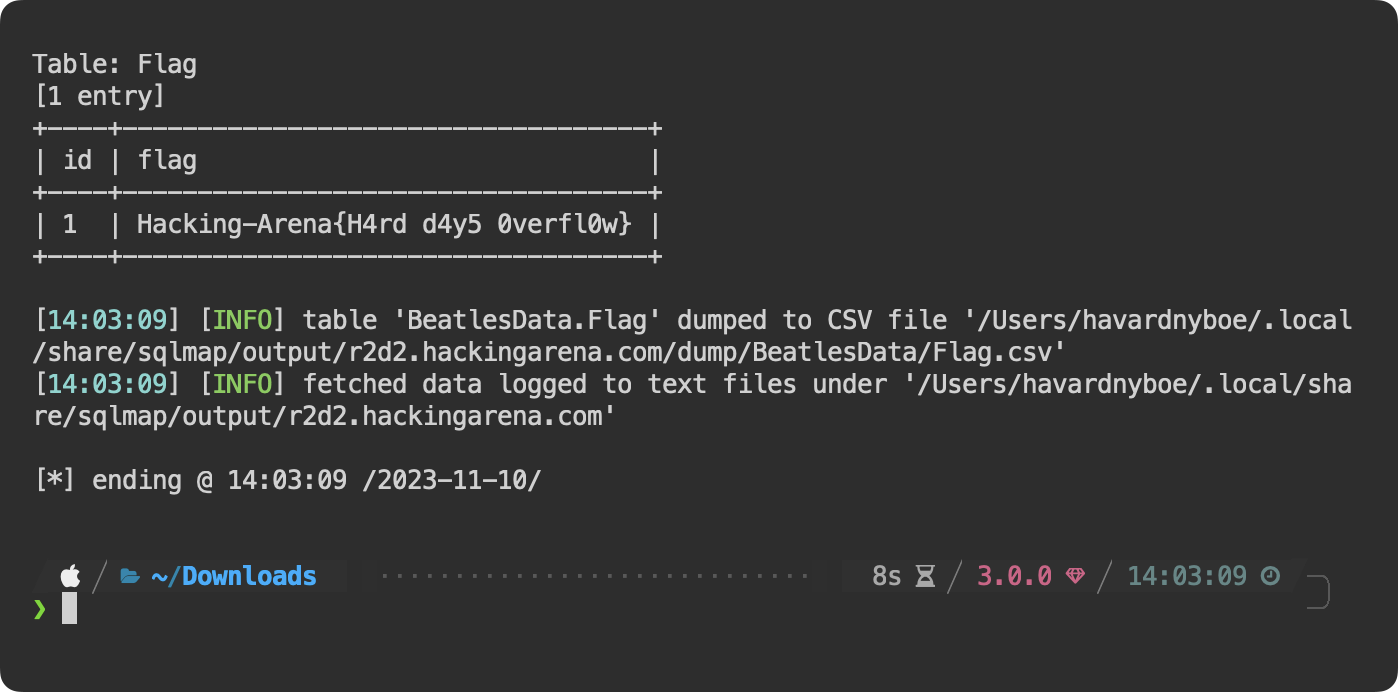
\includegraphics[width=15cm]{img/Web hacking/Beatles song catalogue 2/Screenshot 2023-11-10 at 14.09.55.png}
\end{center}

\newpage
\subsection{Beatles login 2 (120p)}
Find the user: \url{http://vader.hackingarena.com:825}

\textbf{Solution:}\\
I logged in to the site with all the provided usernames and passwords, and noted the different \texttt{beatlesid} parameters. 
To check if the id persisted I tried to log in with the same user twice and saw that the id was the same. 
I then figured the id I was looking for could de searched for with a brute force attack. 
I therefore set up an intruder attack with a payload set from 10000. 
When I realized that it would take a long time using Burp Suite I noticed all the ids for the users were prime numbers. 
So I started another intruder attack with the payload set to prime numbers from 10000. After the attack had ran for a while I found the following page with the id \texttt{17159}:

\begin{center}
    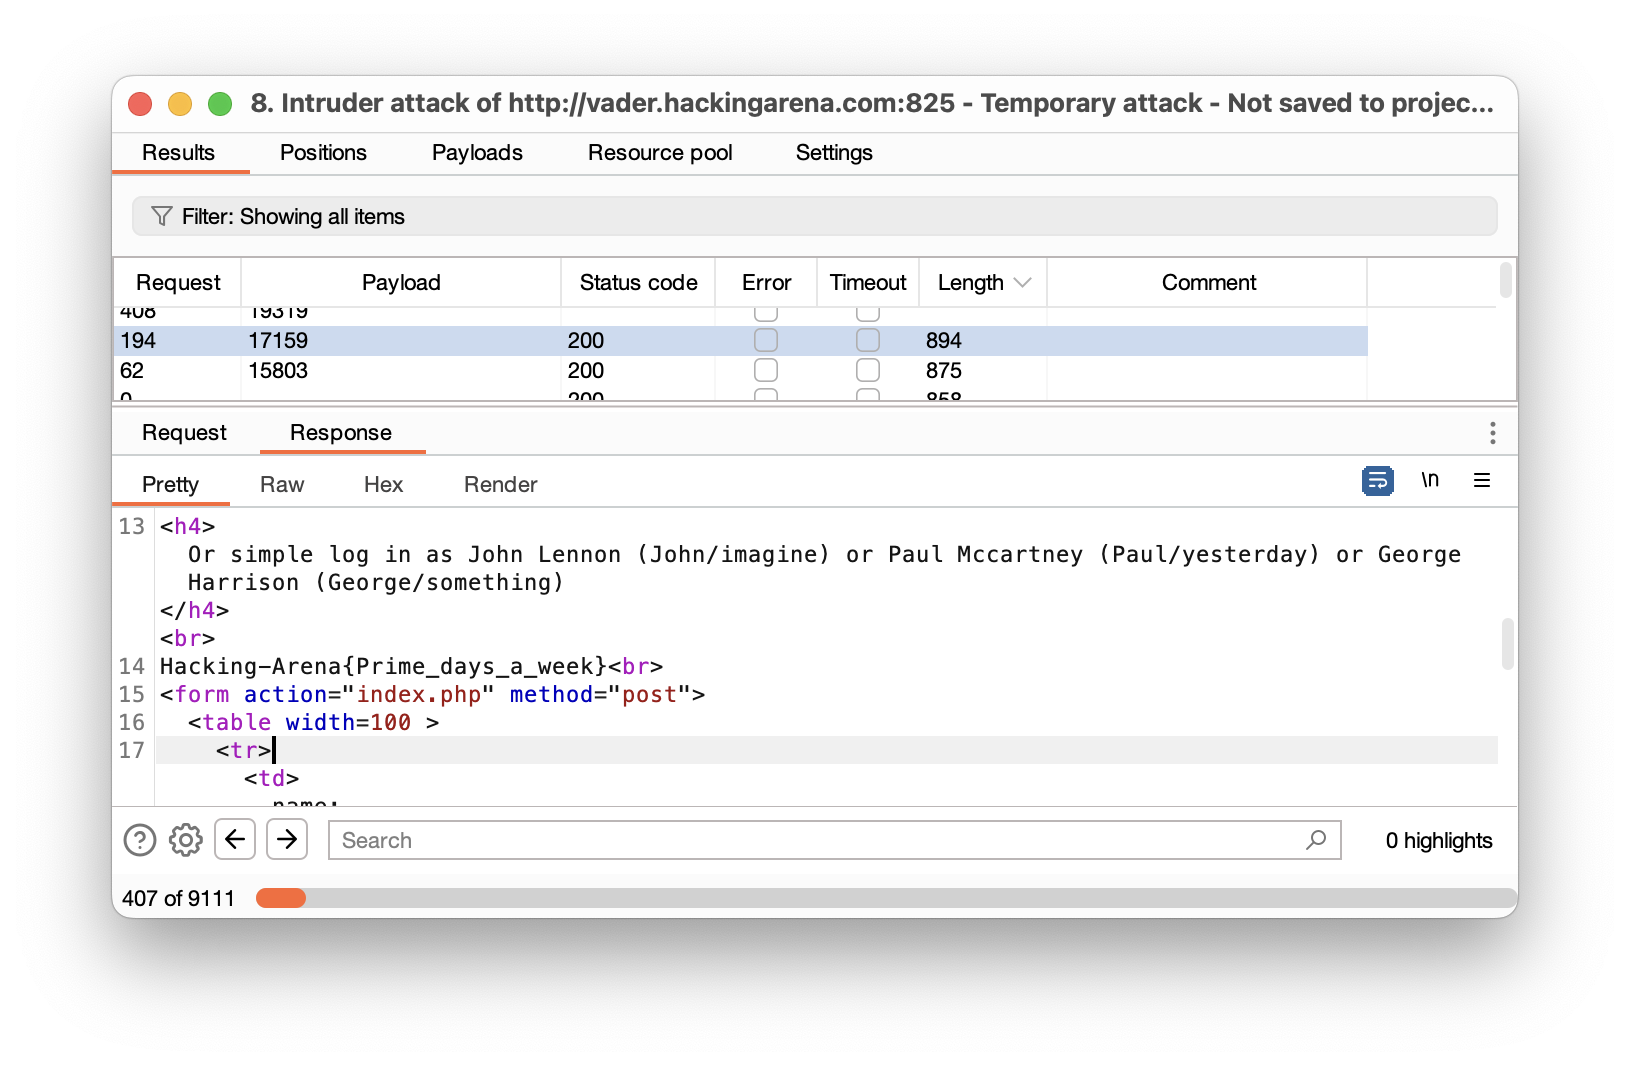
\includegraphics[width=16cm]{img/Web hacking/Beatles login 2/Screenshot 2023-11-09 at 17.33.16.png}
\end{center}

The flag is: \texttt{Hacking-Arena\string{Prime\_days\_a\_week\string}}